%%%%%%%%%%%%%%%%%%%%%%%%%%%%%%%%%%%%%%%%%
% Masters/Doctoral Thesis 
% LaTeX Template
% Version 1.43 (17/5/14)
%
% This template has been downloaded from:
% http://www.LaTeXTemplates.com
%
% Original authors:
% Steven Gunn 
% http://users.ecs.soton.ac.uk/srg/softwaretools/document/templates/
% and
% Sunil Patel
% http://www.sunilpatel.co.uk/thesis-template/
%
% License:
% CC BY-NC-SA 3.0 (http://creativecommons.org/licenses/by-nc-sa/3.0/)
%
% Note:
% Make sure to edit document variables in the Thesis.cls file
%
%%%%%%%%%%%%%%%%%%%%%%%%%%%%%%%%%%%%%%%%%

%----------------------------------------------------------------------------------------
%	PACKAGES AND OTHER DOCUMENT CONFIGURATIONS
%----------------------------------------------------------------------------------------

\documentclass[10pt, oneside]{Thesis} % The default font size and one-sided printing (no margin offsets)

\graphicspath{{Pictures/}} % Specifies the directory where pictures are stored

\usepackage[square, numbers, comma, sort&compress]{natbib} % Use the natbib reference package - read up on this to edit the reference style; if you want text (e.g. Smith et al., 2012) for the in-text references (instead of numbers), remove 'numbers' 
%\usepackage{algpseudocode}
\usepackage{algorithmic}
\usepackage[algoruled]{algorithm2e}
\usepackage{subfigure}
\usepackage{xcolor}
\usepackage{pdfpages}

\newcommand{\continue}{\emph{\color{red}{to be continued...}}}
\newcommand{\todo}[1]{\emph{\color{red}{#1}}}
\newcommand{\blue}[1]{\emph{\color{blue}{#1}}}
\newcommand{\term}[1]{\emph{#1}}
\newcommand{\chref}[1]{Chapter~\ref{#1}}
\newcommand{\xref}[1]{Section~\ref{#1}}
\newcommand{\pxref}[1]{(\xref{#1})}
\newcommand{\alref}[1]{Algorithm~\ref{#1}}
\newcommand{\equref}[1]{Equation~\ref{#1}}
%\newcommand{\fref}[1]{Figure~\ref{#1}}
%\newcommand{\tref}[1]{Table~\ref{#1}}
%\newcommand{\eref}[1]{(\ref{#1})}
\newcommand{\strong}[1]{\textbf{#1}}
\newcommand{\first}{First,~}
\newcommand{\second}{Second,~}
\newcommand{\third}{Third,~}
\newcommand{\fourth}{Fourth,~}
\newcommand{\fifth}{Fifth,~}
\newcommand{\sixth}{Sixth,~}
\newcommand{\ie}{\emph{i.\,e.}, \@}
\newcommand{\eg}{\emph{e.\,g.}, \@}
\newcommand{\Ie}{\emph{I.\,e.}, \@}
\newcommand{\Eg}{\emph{E.\,g.}, \@}
\newcommand{\cf}{\emph{cf.}~}
\newcommand{\Cf}{\emph{Cf.}~\@}
\newcommand{\etal}{\emph{et~al.}\xspace}
\newcommand{\perc}{\,\%\xspace}
\newcommand{\pert}{\,\textperthousand\xspace}

\newcommand{\mhttp}{\emph{mHTTP}}
\newcommand{\algbase}{\emph{Baseline}}
\newcommand{\algalpha}{\emph{Smart $\alpha$}}
\newcommand{\algslice}{\emph{Smart Time Slice}}
\newcommand{\protoold}{\emph{mHTTP Vanilla}}
\newcommand{\protonew}{\emph{Smart mHTTP}}
\newcommand{\wifi}{WIFI}
\newcommand{\ethernet}{Ethernet}
\newcommand{\lte}{LTE}

\hypersetup{urlcolor=blue, colorlinks=true} % Colors hyperlinks in blue - change to black if annoying
\title{\ttitle} % Defines the thesis title - don't touch this

\begin{document}

\frontmatter % Use roman page numbering style (i, ii, iii, iv...) for the pre-content pages

\setstretch{1.0} % Line spacing of 1.3

% Define the page headers using the FancyHdr package and set up for one-sided printing
\fancyhead{} % Clears all page headers and footers
\rhead{\thepage} % Sets the right side header to show the page number
\lhead{} % Clears the left side page header

\pagestyle{fancy} % Finally, use the "fancy" page style to implement the FancyHdr headers

\newcommand{\HRule}{\rule{\linewidth}{0.5mm}} % New command to make the lines in the title page

% PDF meta-data
\hypersetup{pdftitle={\ttitle}}
\hypersetup{pdfsubject=\subjectname}
\hypersetup{pdfauthor=\authornames}
\hypersetup{pdfkeywords=\keywordnames}

%----------------------------------------------------------------------------------------
%	TITLE PAGE
%----------------------------------------------------------------------------------------

\begin{titlepage}
\begin{center}

\textsc{\LARGE \univname}\\[1.5cm] % University name
\textsc{\Large Master Thesis}\\[0.5cm] % Thesis type

\HRule \\[0.4cm] % Horizontal line
{\huge \bfseries \ttitle}\\[0.4cm] % Thesis title
\HRule \\[1.5cm] % Horizontal line
 
\begin{minipage}{0.4\textwidth}
\begin{flushleft} \large
\emph{Author:}\\
%\href{http://fishi.devtail.com}{\authornames} % Author name - remove the \href bracket to remove the link
{\authornames}\\
{\small{319302}}
\end{flushleft}
\end{minipage}
\begin{minipage}{0.4\textwidth}
\begin{flushright} \large
\emph{Supervisor:} \\
{\supname}\\ % Supervisor name - remove the \href bracket to remove the link  
\small{}
\end{flushright}
\end{minipage}\\[1cm]
\begin{minipage}{0.8\textwidth}
\begin{flushright} \large
\emph{Advisor:} \\
Juhoon Kim \\
Ramin Khalili
\end{flushright}
\end{minipage}\\[3cm]
 
\large \textit{A thesis submitted in fulfilment of the requirements\\ for the degree of \degreename}\\[0.3cm] % University requirement text
\textit{in the}\\[0.4cm]
%\groupname\\\deptname\\[2cm] % Research group name and department name
\deptname\\[2cm] % Research group name and department name
 
%{\large \today}\\[4cm] % Date
{\large August 2015}\\[4cm]
%\includegraphics{Logo} % University/department logo - uncomment to place it
 
\vfill
\end{center}

\end{titlepage}

%----------------------------------------------------------------------------------------
%	DECLARATION PAGE
%	Your institution may give you a different text to place here
%----------------------------------------------------------------------------------------

\Declaration{

\addtocontents{toc}{\vspace{1em}} % Add a gap in the Contents, for aesthetics

Hiermit erkläre ich, dass ich die vorliegende Arbeit selbstständig\\
und eigenhändig sowie ohne unerlaubte fremde Hilfe und\\
ausschließlich unter Verwendung der aufgeführten Quellen und Hilfsmittel\\
angefertigt habe.\\[1em]
Berlin, den\\
\vspace{2em}

…………………………………………………\\
Unterschrift

%I, \authornames, declare that this thesis titled, '\ttitle' and the work presented in it are my own. I confirm that:

%\begin{itemize} 
%\item[\tiny{$\blacksquare$}] This work was done wholly or mainly while in candidature for a research degree at this University.
%\item[\tiny{$\blacksquare$}] Where any part of this thesis has previously been submitted for a degree or any other qualification at this University or any other institution, this has been clearly stated.
%\item[\tiny{$\blacksquare$}] Where I have consulted the published work of others, this is always clearly attributed.
%\item[\tiny{$\blacksquare$}] Where I have quoted from the work of others, the source is always given. With the exception of such quotations, this thesis is entirely my own work.
%\item[\tiny{$\blacksquare$}] I have acknowledged all main sources of help.
%\item[\tiny{$\blacksquare$}] Where the thesis is based on work done by myself jointly with others, I have made clear exactly what was done by others and what I have contributed myself.\\
%\end{itemize}
 
%Signed:\\
%\rule[1em]{25em}{0.5pt} % This prints a line for the signature
 
%Date:\\
%\rule[1em]{25em}{0.5pt} % This prints a line to write the date
}

\clearpage % Start a new page

%----------------------------------------------------------------------------------------
%	QUOTATION PAGE
%----------------------------------------------------------------------------------------

%\pagestyle{empty} % No headers or footers for the following pages

%\null\vfill % Add some space to move the quote down the page a bit

%\textit{``Thanks to my solid academic training, today I can write hundreds of words on virtually any topic without possessing a shred of information, which is how I got a good job in journalism."}

%\begin{flushright}
%Dave Barry
%\end{flushright}

%\vfill\vfill\vfill\vfill\vfill\vfill\null % Add some space at the bottom to position the quote just right

%\clearpage % Start a new page

%----------------------------------------------------------------------------------------
%	ABSTRACT PAGE
%----------------------------------------------------------------------------------------

\addtotoc{Abstract} % Add the "Abstract" page entry to the Contents

\abstract{\addtocontents{toc}{\vspace{1em}} % Add a gap in the Contents, for aesthetics
Multi-source Multipath HTTP (\mhttp) is a client oriented mechanism which enables users to
simultaneously download partial chunks of the same content from different servers. The previous
implementation of \mhttp, \ie \protoold, has proven that it takes advantages of different types of network
diversity, \eg Interface diversity, data source diversity, and path diversity, for downloading a large file. 
However, how \mhttp~performs on web pages, \ie downloading a HTML page followed by multiple embedded web objects, is largely uncharted in the previous study.
Furthermore, \protoold~applies a fixed size to all partial blocks of the content during the transfer, which leads to performance issues when the quality of the links changes. 
Link performance changes should be handled by an intelligent algorithm, \ie a scheduler that minimizes the request overhead, while still being adaptive to quality changes of the link. 
Additionally, a path manager which is part of the scheduler should select an optimal path, meaning the determination of a client interface and a server in order to achieve maximum overall throughput.
The major purpose of this thesis is to develop and evaluate efficient scheduling algorithms for \mhttp. 
Key challenges to perform this study are: 
First, to develop \protonew, \ie a prototype that allows multi-file (web page) downloads and a dynamic chunk size. 
Second, to design and implement different scheduling algorithms for \protonew. 
Finally, to evaluate these scheduling algorithms over controlled testbeds and in real-world experiments.


%However, how \mhttp~performs on web pages, \ie downloading a HTML page followed by multiple embedded web objects, is largely uncharted in the previous study. 
%Furthermore, the previous study applies a fixed size to all chunks, \ie partial blocks of content requested by a client, that leads to performance issues when the quality of links changes. 
%Link performance changes should be handled by a scheduler that minimizes request overhead, while still being adaptive to quality changes of the link and that selects an optimal path meaning the selection of a client interface and a server to achieve maximum overall throughput. 

%The Thesis Abstract is written here (and usually kept to just this page). The page is kept centered vertically so can expand into the blank space above the title too\ldots
}

\clearpage % Start a new page

\addtotoc{German Abstract} % Add the "Abstract" page entry to the Contents

\abstractde{\addtocontents{toc}{\vspace{1em}} % Add a gap in the Contents, for aesthetics
Multi-source Multipath HTTP (\mhttp) ist ein Client orientierter Mechanismus, welcher Nutzern erlaubt identischen Content von verschiedenen Servern zur selben Zeit zu laden. 
Die vorherige Implementierung von \mhttp, \protoold, hat bewiesen, dass \mhttp~in der Lage ist verschiedene Arten von Netzwerkvielfalt wie zum Beispiel das Vorhandensein mehrerer Client Interfaces und Datenquellen und die daraus resultierenden Pfade positiv zu nutzen, um große Dateien zu laden. 
Dennoch wurde das Verhalten von \mhttp~bei Website Downloads, d. h. das Herunterladen einer HTML Seite, gefolgt von mehreren eingebetteten Webobjekten, von den bisherigen Studien nicht untersucht. 
Des Weiteren nutzt \protoold~während des Datentransfers eine feste Größe für alle partiellen Blöcke des Contents, was zu Performanceproblemen bei Linkqualitätsänderungen führt. 
Diese Linkqualitätsänderungen sollten durch einen intelligenten Algorithmus behandelt werden, d. h. ein Scheduler, welcher Request Overhead minimiert während er adaptiv zu Linkqualitätsänderungen bleibt.
Zusätzlich muss ein Pfadmanager, welcher Teil des Schedulers ist, einen optimalen Pfad wählen, d. h. ein Client Interface und eine Datenquelle (Server) wählen, um maximalen Datendurchsatz zu erzielen. 
Hauptaufgabe dieser Arbeit ist es effiziente Scheduler Algorithmen für \mhttp~zu entwickeln und zu evaluieren. 
Die Hauptherausforderungen dieser Arbeit sind:
Erstens, \protonew~zu entwickeln, d. h. einen neuen \mhttp~Prototypen zu implementieren, welcher Website Downloads und dynamische Blockgrößen erlaubt. 
Zweitens, verschiedene Scheduler Algorithmen für \protonew~zu entwickeln. 
Drittens, diese Scheduler Algorithmen in einem kontrollierten Testbed und mit real-world Experimenten zu evaluieren. 

%Multi-source Multipath HTTP (\mhttp) is a client oriented mechanism which enables users to simultaneously download partial chunks of the same content from different servers. 
%The previous implementation of \mhttp, \ie \protoold, has proven that it takes advantages of different types of network diversity, \eg Interface diversity, data source diversity, and path diversity, for downloading a large file. 
%However, how \mhttp~performs on web pages, \ie downloading a HTML page followed by multiple embedded web objects, is largely uncharted in the previous study.
%Furthermore, \protoold~applies a fixed size to all partial blocks of the content during the transfer, which leads to performance issues when the quality of the links changes. 
%Link performance changes should be handled by an intelligent algorithm, \ie a scheduler that minimizes the request overhead, while still being adaptive to quality changes of the link. 
%Additionally, a path manager which is part of the scheduler should select an optimal path, meaning the determination of a client interface and a server in order to achieve maximum overall throughput.
%The major purpose of this thesis is to develop and evaluate efficient scheduling algorithms for \mhttp. 
%Key challenges to perform this study are: 
%First, to develop \protonew, \ie a prototype that allows multi-file (web page) downloads and a dynamic chunk size. 
%Second, to design and implement different scheduling algorithms for \protonew. 
%Finally, to evaluate these scheduling algorithms over controlled testbeds and in real-world experiments.

\clearpage

%----------------------------------------------------------------------------------------
%	ACKNOWLEDGEMENTS
%----------------------------------------------------------------------------------------

\setstretch{1.3} % Reset the line-spacing to 1.3 for body text (if it has changed)

\acknowledgements{\addtocontents{toc}{\vspace{1em}} % Add a gap in the Contents, for aesthetics

First and foremost I offer my sincerest gratitude to Juhoon Kim, who supervised and supported me throughout the whole process of working on this topic. 
I attribute the level of my Master's degree to his professional insights and encouragements. 
One simply could not wish for a better or friendlier mentor. 

Further, I want to thank Ramin Khalili, especially because of his great expertise and experience in scheduler algorithm design which greatly helped me during my work on the chunk scheduler algorithms. 

%First and foremost I offer my sincerest gratitude to my direct supervisors, Juhoon Kim and Ramin Khalili, who have supported me throughout my thesis with their patience and knowledge whilst allowing me the room to work in my own way. 
%I attribute the level of my Masters degree to their encouragement and effort and without them this thesis, too, would not have been completed or written. 
%One simply could not wish for better or friendlier supervisors. 

I want to thank Yung-Chih Chen for providing such great help and effort in the measurement process. 
Without him, the measurements in our US testbed could not have been conducted.  

I also want to thank Prof. Anja Feldmann for giving me the opportunity to work on such an amazing topic. 

Last but not the least, I want to thank my parents for supporting me throughout writing this thesis and my life in general.

%I also want to thank Prof. Yuan Bo and Prof. Xiaoyao Liang, who have given me their professional advise and support across continents, which allowed me to finish this thesis according to SJTU standards. 
}
\clearpage % Start a new page

%----------------------------------------------------------------------------------------
%	LIST OF CONTENTS/FIGURES/TABLES PAGES
%----------------------------------------------------------------------------------------

\pagestyle{fancy} % The page style headers have been "empty" all this time, now use the "fancy" headers as defined before to bring them back

\lhead{\emph{Contents}} % Set the left side page header to "Contents"
\tableofcontents % Write out the Table of Contents

\lhead{\emph{List of Figures}} % Set the left side page header to "List of Figures"
\listoffigures % Write out the List of Figures

%\lhead{\emph{List of Tables}} % Set the left side page header to "List of Tables"
%\listoftables % Write out the List of Tables

%----------------------------------------------------------------------------------------
%	ABBREVIATIONS
%----------------------------------------------------------------------------------------

%\clearpage % Start a new page

%\setstretch{1.5} % Set the line spacing to 1.5, this makes the following tables easier to read

%\lhead{\emph{Abbreviations}} % Set the left side page header to "Abbreviations"
%\listofsymbols{ll} % Include a list of Abbreviations (a table of two columns)
%{
%\textbf{LAH} & \textbf{L}ist \textbf{A}bbreviations \textbf{H}ere \\
%\textbf{Acronym} & \textbf{W}hat (it) \textbf{S}tands \textbf{F}or \\
%}

%----------------------------------------------------------------------------------------
%	PHYSICAL CONSTANTS/OTHER DEFINITIONS
%----------------------------------------------------------------------------------------

%\clearpage % Start a new page

%\lhead{\emph{Physical Constants}} % Set the left side page header to "Physical Constants"

%\listofconstants{lrcl} % Include a list of Physical Constants (a four column table)
%{
%Speed of Light & $c$ & $=$ & $2.997\ 924\ 58\times10^{8}\ \mbox{ms}^{-\mbox{s}}$ (exact)\\
% Constant Name & Symbol & = & Constant Value (with units) \\
%}

%----------------------------------------------------------------------------------------
%	SYMBOLS
%----------------------------------------------------------------------------------------

%\clearpage % Start a new page

%\lhead{\emph{Symbols}} % Set the left side page header to "Symbols"

%\listofnomenclature{lll} % Include a list of Symbols (a three column table)
%{
%$a$ & distance & m \\
%$P$ & power & W (Js$^{-1}$) \\
% Symbol & Name & Unit \\

%& & \\ % Gap to separate the Roman symbols from the Greek

%$\omega$ & angular frequency & rads$^{-1}$ \\
% Symbol & Name & Unit \\
%}

%----------------------------------------------------------------------------------------
%	DEDICATION
%----------------------------------------------------------------------------------------

%\setstretch{1.3} % Return the line spacing back to 1.3

%\pagestyle{empty} % Page style needs to be empty for this page

%\dedicatory{For/Dedicated to/To my\ldots} % Dedication text

%\addtocontents{toc}{\vspace{2em}} % Add a gap in the Contents, for aesthetics

%----------------------------------------------------------------------------------------
%	THESIS CONTENT - CHAPTERS
%----------------------------------------------------------------------------------------

\mainmatter % Begin numeric (1,2,3...) page numbering

\pagestyle{fancy} % Return the page headers back to the "fancy" style

% Include the chapters of the thesis as separate files from the Chapters folder
% Uncomment the lines as you write the chapters

\chapter{Introduction} % Main chapter title
\label{ch:introduction}

\lhead{Chapter I. \emph{Introduction}} % Change X to a consecutive number; this is for the header on each page - perhaps a shortened title

%- multiple interfaces / sources, but HTTP does not take advantage of that

%- take advantage of network diversity

%- mHTTP Vanilla already implemented, but not complete for proper evaluations and traffic scheduling


Multi-source Multipath HTTP (\mhttp)~\cite{JKIM14-TUND}\cite{KIMSIG} aims to download a single content from different sources through multiple client interfaces at the same time, intending to reduce the overall download times of web contents for end-users. 
Two major recent developments make such an approach feasible. 
First, the majority of mobile devices has two interfaces (\ie \wifi~and \lte) and 
second, popular content tends to be distributed in Content Distribution Networks (CDN), thus multiple copies of the same popular content exist in several locations. 

Previous studies on \mhttp~\cite{JKIM14-TUND}\cite{KIMSIG} were conducted on single file downloads in controlled testbeds. 
Website downloads and real-world measurements pose a very interesting benchmark to verify, whether \mhttp~indeed has the potential to increase the end-user's every day browsing experience, however, these evaluations are uncharted in the previous studies~\cite{JKIM14-TUND}\cite{KIMSIG}. 
Further, no intelligent chunk scheduling over the available paths was evident, thus different link performances were not considered to leverage the full potential of \mhttp. 

Continuing the previous works~\cite{JKIM14-TUND}\cite{KIMSIG}, we propose a new \mhttp~prototype (\protonew), which is based on the original prototype (\ie \protoold). 
\protonew~comes with the same benefits as its predecessor \protoold, \eg

\begin{itemize}
\item only client socket API modifications are necessary
\item taking advantage of all kinds of network diversities
\item full transparency towards the application layer, \ie applications do not need any special modifications in order to work with \mhttp.
\end{itemize}

In addition to that \protonew~provides 

\begin{itemize}
\item algorithms for intelligent chunk scheduling over the available paths. 
\item an advanced memory management and implementation, allowing to deliver data to the application in less system calls than \protoold.
\item the ability to download websites from servers. 
\item an advanced threading model, enabling quick TCP buffer draining to prevent processing bottlenecks having an effect on the used bandwidth. 
\end{itemize}

In the previous studies~\cite{JKIM14-TUND}\cite{KIMSIG}, each download scenario was repeated several times for different fixed chunk sizes over the paths in order to determine the best performing chunk size. 
Obviously, it is desirable to have an algorithm that automatically figures out the best performing chunk size during download time, without repeating the download and without any prior knowledge about the paths. 
We show that \protonew's intelligent chunk scheduling performs in any download scenario at least as good as the best performing fixed chunk size of \protoold, thus enabling \mhttp~to automatically determine the best traffic distribution during download time without prior knowledge of the paths. 

Moreover, we compare \protonew~to MPTCP and show that it performs similar, thus being a viable alternative. 

Finally, we evaluate \protonew~on popular public websites and show that \mhttp~indeed has the potential of reducing download times for websites with few relatively large embedded objects, while not doing any harm to websites with very small objects only. 



% Background
\chapter{Background} % Main chapter title
\label{ch:background} % Change X to a consecutive number; for referencing this chapter elsewhere, use \ref{ChapterX}

\lhead{Chapter II. \emph{Background}} % Change X to a consecutive number; this is for the header on each page - perhaps a shortened title

We discuss some basic preliminary knowledge that is necessary to fully understand \mhttp~and the chunk scheduling algorithms that we are going to propose in~\chref{ch:scheduler}. 
In more detail we learn about properties of the Hyper Text Transfer Protocol (HTTP), the Domain Name System (DNS), the concept of Content Distribution Networks (CDNs) and congestion avoidance algorithms of the Transmission Control Protocol (TCP).

\section{HTTP}
\label{sec:background-http}

The Hypertext Transfer Protocol (HTTP) is a stateless transfer protocol~\cite{RFC-2616} on top of TCP. 
After establishing a connection to a server, a client forms and sends a request and awaits the response from the server. 
Many different meta parameters about the file and the connection itself can be specified inside a request and response header in order for client and server to properly coordinate the file transfer. 

Currently, HTTP is the most used standard to deploy new services and applications~\cite{defacto-http}.
Estimates state, that HTTP is the main protocol with more than $60$\perc of today's traffic in the internet~\cite{MAIER09-ODC}. 
Moreover, studies have shown that large files are of major importance today, since they account for the bulk of the total volume of traffic on the internet~\cite{MAIER08-ENS}. 
\mhttp~is designed for HTTP traffic and specifically aims to greatly decrease the download times of large files, while not harming download times of very small files.

In order to request only parts of a file, \mhttp~takes advantage of HTTP's range request feature~\cite{RFC-7233}. 
Inside the range request the exact range of wanted bytes can be specified, thus allowing the data to be chunked over different requests. 

\section{DNS}
\label{sec:background-dns}

In order to resolve a human-friendly URL to a set of actual server IP addresses, a Domain Name System (DNS) Server query is required. 
In such a query the client asks its local DNS server to return known IPs for a given URL. 
In case a list of multiple IP addresses is returned, the client usually uses only the first one and discards all other IPs. 
Note, that different DNS servers might return different sets of IPs, \eg results from an ISP's local DNS server might differ from Google's DNS server. 

According to the previous \mhttp~study~\cite{KIM13-MHTTP}, even with a single query to the local ISP's DNS Server, for the top $1000$ websites provided by \term{Alexa.com}~\cite{URL-ALEXA}, approximately $30$\perc are associated to more than one IP address. 
Further, $10$\perc and $5$\perc belong to different network prefixes and different Autonomous Systems (ASes), respectively. 

The study also shows that performing two lookups, one to the local DNS and one to Google's DNS, increases these fractions to $35$\perc (IP addresses), $17$\perc (prefixes) and $7$\perc (ASes). 

Taking advantage of these results is done by \mhttp's \term{MultiDNS} module and is briefly explained in~\chref{ch:vanilla}. 

\section{CDN}
\label{sec:background-cdn}

The goal of Content Distribution Networks (CDNs) is to serve content faster and more reliable to end-users through multiple servers in multiple data centers across the world. 
CDNs provide replication of content and smart matching of end-users to appropriate CDN servers, \eg via PaDIS~\cite{POESE10-ICD} or ALTO~\cite{RFC-ALTO} services, which take advantage of this replication. 
Consequently, this means that the vast majority of popular content is available on multiple sources throughout the Internet. 

Taking advantage of replicated content over multiple sources is one main feature of \mhttp.

\section{TCP}
\label{sec:background-tcp}

TCP applies algorithms, that react to link quality changes and sender/receiver constraints in order to avoid link congestion collapse by limiting the number of sent packets. 
In general, this is called congestion control~\cite{RFC-5681}.

Different algorithms to avoid congestion collapse exist, but all of them have the general idea in common, \ie a congestion window is used to limit the maximum allowed number of unacknowledged packets in end-to-end transit. 
Depending on the link quality, the size of the congestion window changes. 

TCP starts in a slow start phase, \ie the congestion window is very small. 
If no timeout events which signal packet loss occur, TCP rapidly increases the congestion window, assuming the quality of the link is good enough to send more packets. 
After a certain congestion window size threshold is reached, TCP goes into congestion avoidance state, meaning the window from now on increases slower on successful transmissions. 
On loss events the congestion window is decreased, since packet losses are a typical symptom of link overuse. 
Depending on which algorithm is used, the increase and decrease rates of the congestion window differ, but common mechanisms are Linear-Increase/Multiplicative-Decrease or Multiplicative-Increase/Multiplicative-Decrease. 
The first one is usually used during congestion avoidance in order to slowly increase the congestion window.

Besides using congestion control, TCP also limits the sending rate with a flow control algorithm~\cite{RFC-793}. 
A sliding window is applied to determine the maximum possible sender rate at which the receiver's buffer will not be overwhelmed. 
Sender and receiver notify each other about how much data they can buffer, so the opposite end can adjust its sliding window accordingly.
TCP chooses the smaller window from both (congestion and flow control) to limit its sending rate.

Understanding these mechanisms is important in order to develop efficient scheduling algorithms for~\mhttp.


% related work
\chapter{Related Work}
\label{ch:related-work}

\lhead{Chapter III. \emph{Related Work}}

\mhttp~is not the first approach that tries to take advantage of network diversity and deals with chunk scheduling. 
In this chapter we discuss technologies that also try to enhance download speed by using multiple paths, focusing on their chunk scheduling approaches and how we can learn from them.

\strong{Early studies}
One of the early studies by Rodriguez and Biersack~\cite{RODRIGUEZ02-DPA} studies the concept of parallel access to replicated content. 
In their study they use a chunk scheduler that is very similar to \protoold's \algbase~scheduler, which will be further introduced in~\xref{sec:baseline-scheduler}.
Moreover, they mention the problem of idle connections towards the end of a download, thus inspiring us for a connection synchronization approach as introduced in~\xref{sec:synchronization-approach}.

\strong{SCTP}
The Stream Control Transmission Protocol (SCTP)~\cite{IYENGAR06-CMT} enables concurrent multipath transfer. 
Depending on the platform, usually simple scheduler approaches such as Round-Robin or First-Come, First-Serve are used~\cite{RFC-4960}. 
Another study discusses the importance of a pluggable scheduler for easy customizations based on the application need~\cite{YWANG11-INFO}.
This shows that a clean and easy scheduler API can simplify the process of designing and implementing different new scheduling algorithms. 

\strong{MPTCP}
Multipath TCP (MPTCP~\cite{RFC-MPTCP,RAICIU12-HHC}) is a multipath approach between a single server and a single client, which operates on the TCP layer. 
MPTCP Head-Of-Line Blocking, \ie a line of packets blocked by the first one, due to periodic outages on a bad path, is one major concern for optimal scheduling. 
Further, MPTCP might suffer from receive-window limitations, \ie not enough memory to accommodate out-of-order packets~\cite{PAASCH14-MPTCP}. 
Studies have shown, that scheduler algorithms such as Lowest-RTT-First, which take the link quality in terms of round-trip-latency into account, tend to perform better in MPTCP than simple algorithms like Round-Robin~\cite{PAASCH14-MPTCP}.
We discuss important link quality metrics for \mhttp~and how we intent to measure them in~\xref{sec:metrics}. 

\strong{Video streaming}
Studies in video streaming for different providers (\eg Youtube) were performed, in which chunk scheduling algorithms were proposed. 
Evensen~\etal evaluate fixed chunk and dynamic chunk scheduling~\cite{EVENSEN11-ITP}. 
Their video streaming client benefits from dynamic chunk scheduling, because less traffic is distributed on the slow path. 
Chen~\etal propose a dynamic chunk scheduler that doubles or halves the chunk size, based on the evolution of the link quality, \ie the bandwidth~\cite{CHEN14-MMA}. 
Inspired by this, we propose a similar approach that also takes the round-trip-latency and bandwidth into account in~\xref{sec:alpha-approach}. 

%\strong{Download boosters}
%\todo{torrent, JDownloader, samsung galaxy booster}
%\todo{scheduler unknown, but likely simple and very greedy - dishonors the fairness aspect of TCP}

\strong{Socket Intents}
Socket Intents uses pre-configurable policies to decide which interface to use for which kind of traffic~\cite{SCHMIDT13-SIL}. 
It distinguishes between different types of traffic, \eg bulk transfers (big data) and query transfers (small data). 
Depending on the traffic type a primary interface is selected, \eg query transfers preferably over low latency interfaces and bulk transfers preferably over high throughput interfaces. 
In order to accomplish this, the application layer needs to provide additional information about the traffic. 


% mHTTP Vanilla
\chapter{mHTTP Vanilla}
\label{ch:vanilla} 

\lhead{Chapter IV. \emph{mHTTP Vanilla}}

In this chapter we have a brief look at the prototype from previous studies, \protoold. 
The majority of this chapter is already covered by the previous \mhttp~study~\cite{KIM13-MHTTP}, but we have to introduce major components, advantages and potential issues in order to get a deeper understanding of the requirements for the new prototype \protonew. 

\section{Components}
\label{sec:vanilla-components}

\begin{figure*}[t]
		\begin{minipage}[t]{0.5\linewidth}
		\begin{center}
                \subfigure[Regular \mhttp/TCP Stack.]{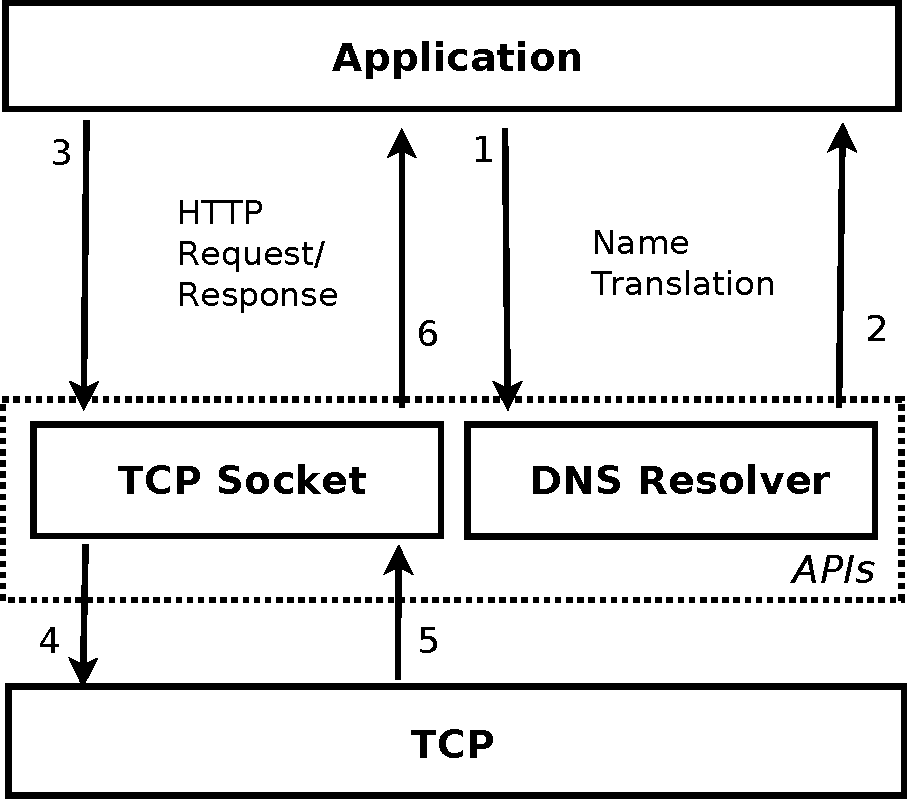
\includegraphics[width=\linewidth]{Figures/http-stack.pdf}}
        \end{center}
        \end{minipage}
~
        \begin{minipage}[t]{0.5\linewidth}
        \begin{center}
                \subfigure[\mhttp Stack on client.]{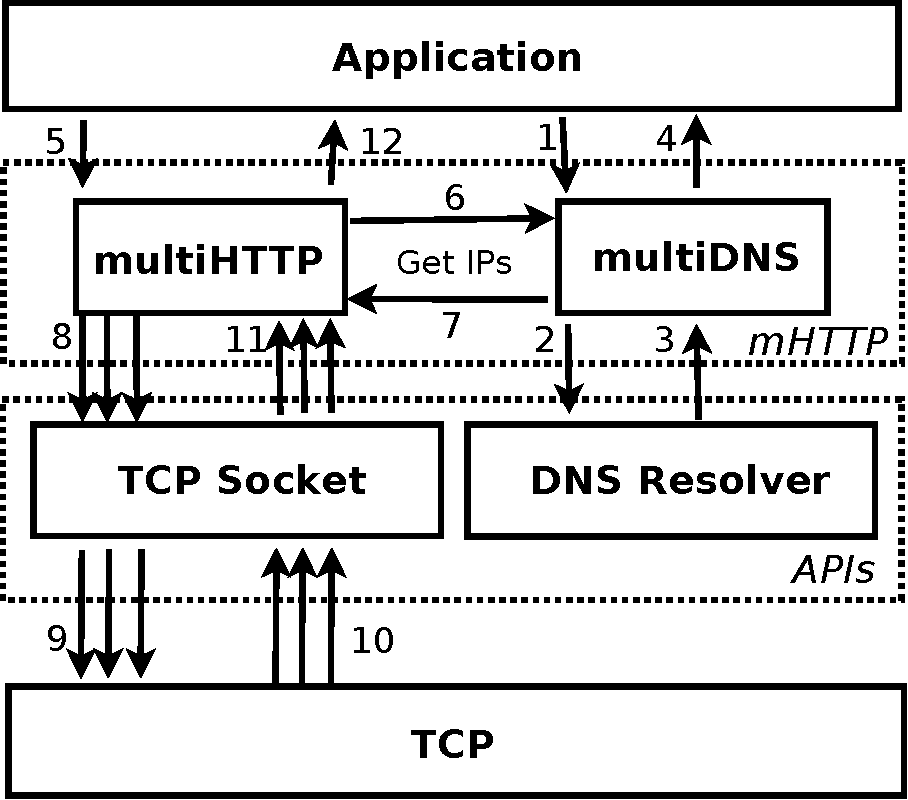
\includegraphics[width=\linewidth]{Figures/mhttp-stack.pdf}}
        \end{center}
        \end{minipage}
        \caption{\label{fig:stack-architecture} Architectural differences between regular HTTP (a) and \mhttp (b) (Figures inspired by previous studies~\cite{JKIM14-TUND}\cite{KIMSIG}\cite{KIM13-MHTTP}).}
  \vspace*{-0.3cm}
\end{figure*}

\mhttp~consists of two major components, \ie \term{multiHTTP} and \term{multiDNS}. 
\fref{fig:stack-architecture} illustrates the major differences between the common HTTP/TCP and the \mhttp~stack. 
We see that \term{multiHTTP} and \term{multiDNS} intercept calls from the application to the TCP layer, in order to manage multiple paths while staying completely transparent towards the application itself. 

\strong{multiHTTP} 
Handling chunked data delivery between the servers and the application is the major purpose of \term{multiHTTP}. 
Further, this module is responsible for the memory management, \ie a buffer in which partial data chunks can be stored even if they arrive out-of-order. 
Moreover, \term{multiHTTP} is responsible for manipulating HTTP request and response headers, \ie removing the response codes of subsequent responses and adding a chunk byte-range to the requests. 

\strong{multiDNS} 
\term{multiDNS} is used to retrieve and keep multiple IP addresses from different DNS servers in different ASes.
Usually an application uses only one server from a DNS query and discards the rest. 
\term{multiDNS} keeps the results of DNS queries from the application and stores all the retrieved IP addresses. 
Consequently, the main task for \term{multiDNS} is to discover and remember as many source servers as possible. 


\section{Advantages}
\label{sec:vanilla-advantages}

\strong{Completely Client Based} \protoold~only requires small changes to the client's socket API. 
Hence, without making any changes to the server, a client can fetch a file from multiple sources at the same time. 
This makes it ideal for studies on download performance of real world content. 

\strong{Transparent to Application Layer} \protoold~is transparent to the application, \ie no changes to the applications have to be done in order to use \mhttp, since it simply wraps around the socket library, while serving the same API. 

\strong{Taking Advantage of different Network Diversities} Using multiple sources and interfaces, \mhttp~takes advantage of the network diversity over different paths.

\section{Problems}
\label{sec:vanilla-problems}

After discussing the advantages of \protoold~we now have a closer look at potential issues. 
Goal of this work is to solve these problems while still maintaining the previously discussed advantages in~\xref{sec:vanilla-advantages}. 

\subsection{Website Download}
\label{sec:problem-website}

In order to download a website an application first has to download an entry document (\eg index.html), which then links to other files such as Cascading Style Sheets (.css), Image files (\eg .png or .jpg) or JavaScript files (.js) that are needed to properly display the website. 

In addition to this, portion of the website content might be dynamic or some static resources might differ on different sources. 
Both of these issues are explained in more detail in~\xref{sec:dynamic-content}.

Further, a raising number of providers uses the Secure Socket Layer (SSL) to secure their websites. 
\protoold~crashes on SSL requests, thus making it very difficult to evaluate popular real-world content. 

Finally, \protoold~is designed to download single files from multiple sources. 
In order to study the performance of \mhttp~on public websites it is important for \protonew~to be able to properly download websites including all their embedded objects. 

\subsection{Intelligent Chunk Scheduling}
\label{sec:problem-static-size}

\protoold~uses a static chunk size, meaning that each chunk has the same size, no matter over which path it is scheduled. 
Obviously, a sophisticated chunk scheduler needs to be able to change chunk sizes for different paths over time in order to optimally distribute the traffic in the network. 

Main contribution of \protonew~is the design and implementation of an intelligent chunk scheduler with a dynamic chunk size, \ie a scheduler that determines the best chunk size for each subsequent request (chunk) to achieve optimal throughput performance. 


% mHTTP Dynamic
\chapter{Smart mHTTP}
\label{ch:scheduler}

\lhead{Chapter V. \emph{Smart mHTTP}}

Intelligent chunk scheduling is a key feature to maximize the overall throughput that can be achieved with \mhttp, which is why 
one major contribution of this work is the design and implementation of such intelligent chunk scheduling algorithms. 
In this chapter we explain in detail the problems of chunk scheduling in \mhttp~and introduce different approaches on how to solve them. 

\protoold~already provides a simple scheduling algorithm with a fixed chunk size, which we call from now on the \algbase~scheduler. 
We will use this scheduler to have a fair baseline comparison with more advanced scheduling approaches. 
%Besides having a fixed chunk size, the \algbase~scheduler tries to determine possible bottleneck connections by comparing the measured throughputs.
%In case a connection is determined as slow and therefore presents a possible bottleneck, the scheduler estimates how many chunks should be skipped by this connection and left for download for the faster connection in order to avoid too many out-of-order chunks in the buffer.

\section{Core Problem}
\label{sec:core-problem}

In order to optimally schedule chunks over multiple connections we must differ between $2$ core problems:

\begin{itemize}
\item \term{Chunk Scheduling}
\item \term{Path Management}
\end{itemize}

When talking about \term{Chunk Scheduling} we mean making a decision for the next range $s$ to be requested over connection $c$. 
We will refer to the request range $s$ from now on as chunk size or chunk request, since the request range at the same time divides our web object into partial blocks of data. 

\begin{figure*}[t]
        \begin{minipage}[t]{0.5\linewidth}
		\begin{center}
                \subfigure[Bad Chunk Scheduling: Assuming $c_2$ has a higher throughput than $c_1$, here the better path has idle time due to bad scheduling towards the end of the file.]{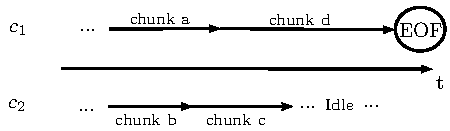
\includegraphics[width=\linewidth]{Figures/scheduler-why-1.pdf}}
        \end{center}
        \end{minipage}
~
        \begin{minipage}[t]{0.5\linewidth}
        \begin{center}
                \subfigure[Bad Path Management: Assuming $c_2$ has a higher throughput than $c_1$, here the better path has idle time due to a bad initial path choice.]{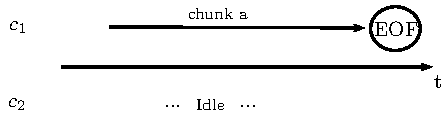
\includegraphics[width=\linewidth]{Figures/path-manager-why-1.pdf}}
        \end{center}
        \end{minipage}
        \caption{\label{fig:bad-scheduling} Illustration of bad chunk scheduling (a) and bad path choices (b).}
  \vspace*{-0.3cm}
\end{figure*}

\term{Path Management} refers to deciding which end-points to use for a new connections, \ie which client network interface and which server (IP) should connect.
Further, in case of website downloads we have to decide which paths we reuse. 
Choosing a bad performing path over a good performing one results in throughput loss and must be avoided. 
In~\xref{sec:path-management} we discuss in more detail our approaches for efficient \term{Path Management}.

In order to visualize the importance of solving these two problems, we illustrate cases of bad \term{Chunk Scheduling} and \term{Path Management} in~\fref{fig:bad-scheduling}. 

In~\fref{fig:bad-scheduling} (a) we illustrate how bad chunk scheduling can have a negative impact on the overall throughput. 
In this case a decision is made so that the slow connection $c_1$ starts downloading chunk $d$ which turns out to be the last block until EOF (end of file).
The decision is done while the fast connection $c_2$ still downloads chunk $c$ and this results in $c_2$ being idle for some time. 
A scenario like that might occur when the link throughput of $c_1$ drops unexpectedly while the assigned chunk size was too big, thus resulting in a much higher download time than expected. 
Especially in heavily used wireless environments rapidly time varying channel conditions are common and have to be taken into account.

Moreover, note that each HTTP request introduces an overhead consisting of a request and a response header, plus one round-trip-latency $rtl$ that is necessary to send the first request byte and receive the first response byte. 
Consequently, each chunk in \mhttp~introduces a request overhead. 
The overall goal of \term{Chunk Scheduling} is to have a minimum request overhead while still maintaining a certain adaptivity towards link changes. 
We see that being adaptive to link changes is of major importance since it is our goal to use each interface to its fullest throughput potential. 

Hence, for optimal \term{Chunk Scheduling} we have to keep two major key issues in mind:

\begin{itemize}
\item a small chunk size leads to higher link adaptivity, but at the same time increases the overall overhead
\item a big chunk size leads to less overhead, but at the same time reduces the overall link adaptivity
\end{itemize}

In~\fref{fig:bad-scheduling} (b) the impact of bad \term{Path Management} is illustrated. 
We see that in case of a small file, initially using the bad connection might lead to a scenario in which the good connection is never used and stays idle. 
This might especially occur in case of website downloads, since here many small files might be sequentially downloaded from the same domain. 
Hence, given we already used different paths and measured their performance, it is important to reuse the good over the bad performing ones. 

\section{Baseline Scheduler}
\label{sec:baseline-scheduler}

\protoold~comes with a very basic chunk scheduler, which requests chunks of a predefined fixed size over each available path. 
During the download this chunk size never changes. 
%Depending on the throughput estimate, some chunks might be skipped by a slow connection in order to avoid too many chunks to arrive out-of-order at the client~\cite{KIM13-MHTTP}. 
Besides having a fixed chunk size, the \algbase~scheduler tries to determine possible bottleneck connections by comparing the measured throughputs from each.
In case a connection is determined as slow and therefore presents a possible bottleneck, the scheduler estimates how many chunks should be skipped by this connection and left to download by the faster connection in order to avoid too many out-of-order chunks in the buffer~\cite{KIM13-MHTTP}.
Hence, the overall goal of this mechanism is to reduce the size of the \mhttp~client chunk buffer. 

%This scheduler is reimplemented in \protonew~in order to have a baseline to compare new scheduler algorithms to. 

As discussed in the previous section, \mhttp~introduces a request overhead for each chunk. 
This can have significant impact on the performance of \mhttp, especially when the chunk sizes are small. 
However, using fixed and large chunk sizes is not recommended as it reduces the responsiveness of \mhttp~towards changes on the network (\eg the throughput and the latency of the connections can greatly vary over time). 
Moreover, requesting chunks of a large fixed size over all connections increases the risk that only the slow connection is active at the end, as the other connection may already have completed the download of its last chunk. 
In the next sections, we propose algorithms that determine and change the sizes of chunks requested over different paths. 
These schedulers measure the performance (\ie throughput and latency) of each of the connections and know the remaining file size that needs to be downloaded from the servers. 
They use all these information to determine the size of the chunk to be downloaded next over a connection.

\section{Smart $\alpha$ Scheduler}
\label{sec:alpha-approach}

As a first dynamic chunk size approach we propose \algalpha, \ie a scheduling algorithm, which dynamically adjusts the chunk size $s$ based on measured throughput and latency changes similar to how TCP handles link congestion. 
In~\xref{sec:background-tcp}, the necessary TCP background knowledge in flow- and congestion-control is explained to fully understand our approach. 

The key idea is that when a link is loosing in quality TCP will adjust the server's sending rate and this might result in a change of the throughput rate at the \mhttp~client. 
When measuring the throughput rate at the client over time we can detect these changes and adjust our chunk size accordingly, thus taking advantage of TCP's optimized link quality estimates. 

In the following we introduce our algorithm for two active connections for simplicities sake, but the algorithm can be easily converted to the scenario that involves more than two connections.

Let $c_1$ and $c_2$ be the connections established by \mhttp. 
We denote by $\overline{R}_i$ and $\overline{rtl}_i$ the estimated throughput and latency (round trip) of $c_i$, and by $s_{i,j}$ the size of the $j$th chunk to be transmitted over $c_i$. 
In~\xref{sec:metrics} we explain in more detail how $\overline{R}_i$ and $\overline{rtl}_i$ are estimated. 

We determine the chunk size $s_{i,j}$ through:

$$s_{i,j}=\alpha_i \cdot \overline{rtl}_i \cdot \overline{R}_i$$

$\alpha_i$ is a value that adjusts based on the evolution of the throughput $\overline{R}_i$. 
This approach is very similar to TCP's congestion window adjustments as discussed in~\xref{sec:background-tcp}. 
Basically $s_{i,j}$ is $\alpha_i$ multiples of bytes that are estimated to be received during $\overline{rtl}_i$. 

We introduce $\alpha_{init}, \delta_{inc}$ and $\delta_{dec}$, which are chosen experimentally and will influence how $\alpha_i$ increases or decreases over time. 
Currently, $\delta_{inc}$ and $\delta_{dec}$ are set to $2$ and $0.9$ respectively. 
The optimal values for these two variables need to be investigated closer in further mobility studies as discussed in~\chref{ch:discussion}.

Given a series of throughput measurements $R_i(t)$, where $t=0,1,\cdots,n-1$, 
we use a Linear Increase / Multiplicative Decrease approach in order to slowly increase and quickly decrease $\alpha_i$, meaning 
$\alpha_i$ is increased linearly by $\delta_{inc}$ if the currently measured throughput $R_{i}(n)$ is sufficiently larger\footnote{Sufficiently means larger than $\gamma \cdot R_{i}(n-1)$, where $\gamma=1.01$} than the previously measured value $R_{i}(n-1)$ or was already decreased in the previous calculation. 
In any other case $\alpha_i$ is multiplicatively decreased by $\delta_{dec}$. 
Through the use of a \term{DECREASED} Flag the algorithm avoids two consecutive decreases in a row, thus an endless decrease spiral is impossible, since after every decrease at least one increase needs to occur. 
Note, that our prototype does not support request pipelining yet which results in a certain idle time between receiving payload blocks.
The \term{DECREASED} Flag is important, since due to wrong estimates we might otherwise schedule very small chunks, which results in more idle times and might decrease the overall sender rate. 
When bad link quality occurs, it is still possible for the scheduler to decrease to a very small chunk size though, since multiplicative decrease evolves faster than linear increase.

We summarize the calculation of $\alpha_i$ in~\alref{alg:dynamic-alpha}.

\begin{algorithm}
\caption{\algalpha~Algorithm}
\label{alg:dynamic-alpha}
\begin{algorithmic}
\STATE{Init: $DECREASED \gets FALSE$}
\STATE{$\gamma \gets 1.01$}
\STATE{$\delta_{dec} \gets 0.9$}
\STATE{$\delta_{inc} \gets 2$}
\IF{$n = 0$}
	\STATE{$\alpha_i \gets \alpha_{init}$}
\ELSE
	\IF{$\gamma \cdot R_{i}(n-1) < R_{i}(n)$ \OR $DECREASED$}
		\STATE{$\alpha_i \gets \alpha_i + \delta_{inc}$}
		\STATE{$DECREASED \gets FALSE$}
	\ELSE
		\STATE{$\alpha_i \gets \delta_{dec} \cdot \alpha_i$}
		\STATE{$DECREASED \gets TRUE$}
	\ENDIF
\ENDIF
\end{algorithmic}
\end{algorithm}

One thing to consider when using this approach is that TCP starts with a very small congestion window, meaning the full capacity of the link is not used initially. 
As already mentioned there exists a certain idle time between receiving payload blocks. 
It follows that if our requested chunk sizes are very small, the TCP congestion window might not grow to its full potential and thus we would waste throughput performance. 
Hence, it is desirable to keep the $\alpha$ value relatively high and to not choose $\alpha_{init}$ too small.

Further, note that the very first chunk over a new connection $c_i$ has a predefined initial chunk size of $32$KB. 
This is due to the fact that initially we have no link estimates yet. 
After receiving this initial chunk we have link quality estimates to make better decisions. 

\begin{figure*}[t]
		\begin{minipage}[t]{0.5\linewidth}
		\begin{center}
                \subfigure[Chunk size evolution of \algalpha.]{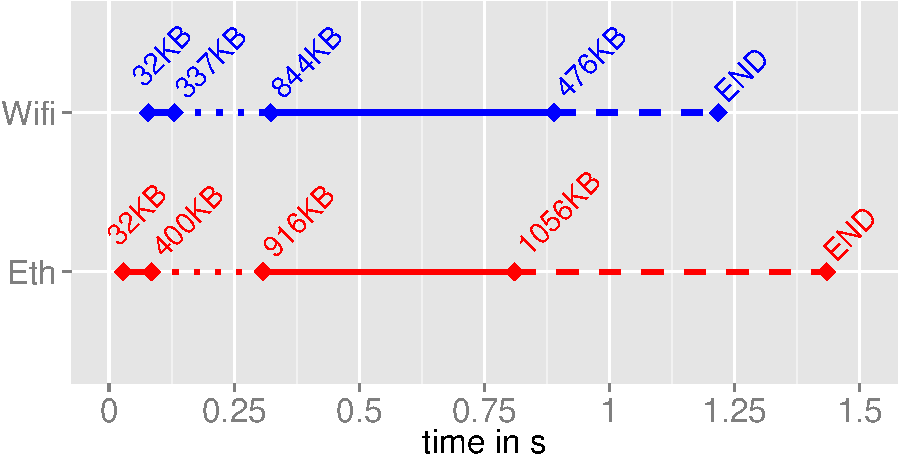
\includegraphics[width=\linewidth]{Figures/flow-dynamic-alpha.pdf}}
        \end{center}
        \end{minipage}
~
        \begin{minipage}[t]{0.5\linewidth}
        \begin{center}
                \subfigure[Chunk size evolution of \algslice.]{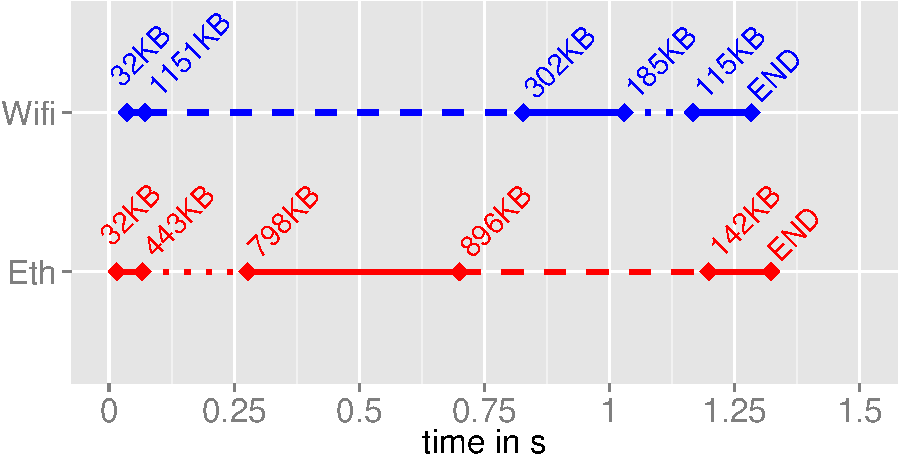
\includegraphics[width=\linewidth]{Figures/flow-dynamic-slices.pdf}}
        \end{center}
        \end{minipage}
        \caption{\label{fig:scheduler-flows} Illustrative examples of how the chunk sizes evolve in case of a $4$MB file download with the \algalpha~scheduler (a) and with the \algslice~scheduler (b).}
  \vspace*{-0.3cm}
\end{figure*}

In~\fref{fig:scheduler-flows} (a) we see an illustrative example of how the chunk sizes evolve on a $4$MB file download with the \algalpha~scheduler. 
We can see how the chunk sizes are getting bigger shortly after the initial chunks, since our throughput estimates are rising and more accurate. 
The first chunk for each connection is the predefined initial chunk size of $32$KB. 
Later the difference between the chunk sizes of each connection is due to the different measured link qualities. 
We can also clearly see that the last chunk of the \wifi~connection is much smaller than the previous one. 
This is due to the fact that we reached the end of the file and there are no more chunks to request. 
This example illustrates very good that we successfully achieve a variable chunk size based on the link quality. 
Moreover, it illustrates an essential problem that still needs to be solved, \ie in the end the \wifi~connection stays idle for a relatively long time. 
It is desirable to synchronize the last chunk download of each connection to avoid such idle times. 
In~\xref{sec:synchronization-approach} we propose an algorithm that solves this problem. 

\section{Smart Time Slice Scheduler}
\label{sec:synchronization-approach}

Using \algalpha~ensures an adaptiveness to link quality changes. 
Still, this algorithm does not take into account bad chunk scheduling decisions for end-of-file scenarios as depicted in~\fref{fig:bad-scheduling} (a). 
In this section we introduce the \algslice~algorithm, which takes such end-of-file scenarios into account. 

Key idea of this scheduler is that in order to optimally bundle the throughput performance of each active path we have to optimize the path synchronization. 
Path synchronization means that the traffic should be distributed in a way such that each path finishes downloading its very last chunk at the same time, keeping each path busy and thus reducing unnecessary idle times.
We propose a scheduling algorithm whose goal is to determine an optimal download time span for each chunk. 
Together with the throughput and round-trip-time estimates of each active path we can determine a chunk size for optimal path synchronization.

In the following we introduce our algorithm for two active connections for simplicities sake, but the algorithm can be easily converted to also work with more than two connections.

Let $c_1$ and $c_2$ be the connections established by \mhttp. 
We define $\overline{R}_i$ and $\overline{rtl}_i$ as the estimated throughput and latency (round trip) of $c_i$, and by $s_{i,j}$ we denote the size of the $j$th chunk to be transmitted over $c_i$. 
In~\xref{sec:metrics} we explain in detail how $\overline{R}_i$ and $\overline{rtl}_i$ are estimated.
The task of the scheduler is to determine $s_{i,j}$ upon the completion of the download of the $(j-1)$-th chunk.

%Chunk scheduling means making decisions for the size of each request range $s_{i,j}$ with $j=1,2,3 \cdots, n$ for a connection $c_{i}$. 


%We define $R_i$, $rtt_i$ and $T_{i,j}$ as the estimated throughput and round-trip-time of connection $i$ and the estimated optimal time span of chunk $j$ for connection $i$ repsectively. 
%We use harmonic mean to estimate the trhoughput $R_i$ on every socket read operation. 
%Given a series of bandwidth measurements $\overline{R}_i(t)$, where $t=0,1,2,\cdots, n-1$, the harmonic mean can be calculated with
%(TODO: ref Yung-Chih Paper):
%
%$$R_i = \frac{n+1}{\frac{n}{R_i} + \frac{1}{\overline{R}_i(n+1)}}$$

%The round-trip-time $rtt_i$ is estimated on every received response header with a moving average as described in section~\ref{sec:metrics}. 
%The optimal $j$th chunk size of connection $i$, $s_{i,j}$ is defined as: 

%$$s_{i,j} = R_i \cdot T_{i,j}$$

\begin{figure*}[t]
		\begin{minipage}[t]{0.3\linewidth}
		\begin{center}
                \subfigure[Scheduler $\beta$: For $c_1$ the closest estimated time $\beta_{i,j}$ until another connection finishes downloading its current chunk.]{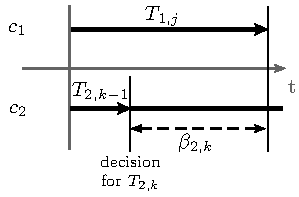
\includegraphics[width=\linewidth]{Figures/scheduler-beta.pdf}}
        \end{center}
        \end{minipage}
~
        \begin{minipage}[t]{0.3\linewidth}
		\begin{center}
                \subfigure[Scheduler Case 1: $c_1$ can download the remaining bytes in the next request while staying within its upper boundary $T_{1,max}$ and before $c_2$ finishes downloading its current chunk.]{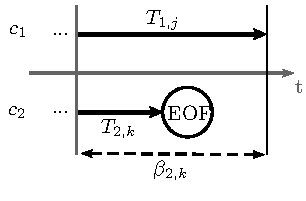
\includegraphics[width=\linewidth]{Figures/scheduler-case-1.pdf}}
        \end{center}
        \end{minipage}
~
        \begin{minipage}[t]{0.3\linewidth}
        \begin{center}
                \subfigure[Scheduler Case 2: $c_1$ and $c_2$ need to make one more request each to download the remaining bytes while staying within their upper boundaries $T_{1,max}$ and $T_{2,max}$.]{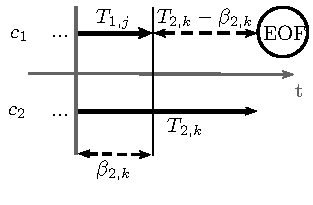
\includegraphics[width=\linewidth]{Figures/scheduler-case-2.pdf}}
        \end{center}
        \end{minipage}
        \caption{\label{fig:scheduler-cases} The $\beta$ value and illustrated Scheduler Cases 1 (b) and 2 (c): Both cases are close to the end of the file, meaning $c_1$ and $c_2$ can download the remaining bytes in their next requests while staying within their upper request limits $T_{1,max}$ and $T_{2,max}$.}
  \vspace*{-0.3cm}
\end{figure*}

Let $T_{i,j}$ be the time to transmit the $j$-th chunk over $c_i$; we have
\begin{equation}
\label{eq:time}
T_{i,j} = s_{i,j} / \overline{R}_i,
\end{equation}
In order to simplify our algorithm design, we assume that $\overline{R}_i$ does not change during the transmission of the $j$-th chunk, while $T_{i,j}$ is calculated. 

As discussed before in~\xref{sec:core-problem}, \mhttp~introduces a delay each time it performs a range 
request over a connection. This delay equals half of the latency of the connection, \ie the 
time that it takes for the HTTP range request to reach the server. Hence, the 
effective throughput $E_i$ of $c_i$, during the transmission of the $j$-th chunk, can be 
estimated as 
$$E_i = \frac{s_{i,j}}{T_{i,j} + 0.5 \overline{rtl}_i}$$
Let $T_{i,j} = \alpha_{i,j} \cdot \overline{rtl}_i$. Using \equref{eq:time}, we have
$$E_i=\frac{\alpha_{i,j} \cdot \overline{R}_i}{\frac{1}{2} + \alpha_{i,j}}.$$ 
$\alpha_{i,j}$ should be sufficiently large so that the effective throughput is larger than a certain 
threshold. In particular, with $\alpha_{i,j}=20$ we can ensure that $E_i > 0.975 \cdot \overline{R}_i$. 
Therefore, we set $T_{i,max}=20 \cdot \overline{rtl}_{i}$ as the maximum value for $T_{i,j}$ . 
In the other term, using our algorithm, we do not request chunks larger than 
$s_{i,max}=20 \cdot \overline{R}_i \cdot \overline{rtl}_{i}$, as requesting larger chunks does not bring
a significant gain. 

In order to avoid the connection idle times towards the end of the download, a special attention needs to be paid when assigning the size of the last chunks over each path to guarantee that the downloads of these last chunks complete at {\it roughly} the same time. 

Let $L$ be the size of the file and $\delta$ the amount of data that has been already 
downloaded/requested. Further, let $\beta_{i,j}$ be the time between the $j$-th scheduling 
decision for $c_i$ and the estimated time until the other connection completes its current 
download (see~\fref{fig:scheduler-cases} (a)).\footnote{$\beta_{i,j}$ is set to infinity if $c_i$ is the only 
established connection.} 
We consider four cases when determining the size of the next chunk 
over $c_i$. We specify the value of $T_{i,j}$ in each of these cases (note that $s_{i,j} = \overline{R}_i \cdot T_{i,j}$). 
Without loss of generality, we focus on the case where the scheduler wants to determine the next chunk for $c_2$. 

\begin{itemize}
\item Case 1 (\fref{fig:scheduler-cases}(b)): $c_2$ can download all remaining $L-\delta$ bytes  
within a time less than $T_{2,max}$ and before the other connection completes its current chunk download, 
\ie $\overline{R}_2 \cdot \beta_{2,j} \geq L-\delta$ and $ \overline{R}_2 \cdot T_{2,max} \geq L-\delta$. In this case, $T_{2,j}$ is the 
time required to download $L-\delta$, \ie $T_{2,j} = \frac{L-\delta}{\overline{R}_2}$.

\item Case 2 (\fref{fig:scheduler-cases} (b)): $\overline{R}_2 \cdot \beta_{2,j} < L-\delta$, but there exists a $T_{2,j} \leq T_{2,max}$ such that  
%but none of them can download $L-\delta$ in a single request. 
%In this case $T_{1,j}$ is the time in which $c_1$ is likely to finish with $c_2$'s upcoming time slice $T_{1,j} - \beta_{1,j}$:
%In the other term, there exists a $T_{i,j} \leq T_$ 
$$T_{2,j} \cdot \overline{R}_2 + (T_{2,j} - \beta_{2,j}) \cdot \overline{R}_1 = L-\delta.$$
In this case, the scheduler sets 
\begin{equation}
\label{eq:case2}
T_{2,j} = \frac{L-\delta + \beta_{2,j}\cdot \overline{R}_1}{\overline{R}_1 + \overline{R}_2}
\end{equation}
to guarantee that $c_1$ and $c_2$ complete their last chunk download at the same time.

\item Case 3: $\frac{L-\delta + \beta_{2,j}\cdot \overline{R}_1}{\overline{R}_1 + \overline{R}_2} > T_{2,max}$, 
hence, at least three more chunks will need to be fetched over $c_1$ and 
$c_2$ to download the remaining $L-\delta$ bytes. In this case, the maximum 
allowed time span is assigned in order to keep the request overhead low, \ie
$$T_{2,j} = T_{2,max}$$

\item Case 4: $c_2$ is a newly established connection ($j=1$). 
As the scheduler is not aware of the quality of the connection, it 
performs a range request for a relatively small chunk in order to probe the path quality. 
We denote by $initial$ the maximum size of the initial chunk that is allowed 
to be transmitted over a newly established connection; then $s_{2,1}=\min\{initial, L-\delta\}$. 
The value of $initial$ is an input to our scheduler. 
\end{itemize}
Algorithm~\ref{alg:advanced-scheduling} summarizes our scheduler design.

%This reduces the chunk size scheduling problem to only determining an optimal time span $T_{i,j}$.

%We define $\beta_{i,j}$ as the time span between the $j$th scheduling decision of path $i$ and the closest estimated time until another connection finishes downloading its current chunk, as depicted in figure \ref{fig:scheduler-cases} (a). 
%Further we need to determine the maximum allowed time span $T_{i,max}$ for a chunk scheduled over connection $i$, in order to establish an upper limit for a scheduled time slice: 

%$$T_{i,max} = \alpha \cdot rtt_i$$

%where our experiments showed that $\alpha$ should be a value between 20 and 30. 
%This is derived from calculations of the effective throughput $E_i$ of a connection $c_i$. 
%It is the throughput that takes into account the overhead of chunking the data, thus sending more requests and it is defined as the number of transmitted bytes during $\alpha \cdot rtt_i$ divided by the total transmission time on connection $c_i$, $\Omega_i$:

%$$E_i = \frac{\alpha \cdot rtt_i \cdot R_i}{\Omega_i}$$

%where the total transmission time $\Omega_i$ can be calculated through:

%$$\Omega_i = \alpha \cdot rtt_i + 0.5\cdot rtt_i$$

%Putting both equation together we get for the effective throughput:

%$$E_i = \frac{\alpha \cdot R_i}{\frac{1}{2} + \alpha}$$

%When trying to achieve an effective throughput $E_i$ of $\gamma$\% of the physical throughput $R_i$, we can calculate: 

%$$\frac{\alpha \cdot R_i}{\frac{1}{2} + \alpha} = \gamma \cdot R_i $$
%$$\Rightarrow \alpha = \frac{1}{2(\frac{1}{\gamma} - 1)}$$

%Lets say $E_i$ should be at least 95\% of $R_i$, we can calculate that $\alpha$ has to be at least 9.5 to achieve that goal.

%Given a file size $L$, an already downloaded amount of bytes $\delta$ from that file and a round-trip-time estimate $rtt_i$ for a connection $c_i$, when determining the optimal download time span $T_{i,j}$ we distinguish between three cases: \newline 
%\begin{itemize}
%\item Case 1 as depicted in \ref{fig:scheduler-cases}: The connection $c_1$ could download all remaining bytes $L-\delta$ within its upper limit $T_{1,max}$ and before $c_2$ finishes downloading its chunk. 
%In this case $T_{1,j}$ is the time necessary for $c_1$ to download $L-\delta$:

%$$T_{1,j} = \frac{L-\delta}{R_1}$$

%\item Case 2 as depicted in \ref{fig:scheduler-cases}: $c_1$ and $c_2$ could download $L-\delta$ within their next requests while staying inside their upper limits $T_{1,max}$ and $T_{2,max}$ respectively, but none of them could download $L-\delta$ in a single request.
%In this case $T_{1,j}$ is the time in which $c_1$ is likely to finish with $c_2$'s upcoming time slice $T_{1,j} - \beta_{1,j}$:

%$$T_{1,j} \cdot R_1 + (T_{1,j} - \beta_{1,j}) \cdot R_2 = L-\delta$$
%$$\Rightarrow T_{1,j} = \frac{L-\delta + \beta_{1,j}\cdot R_2}{R_1 + R_2}$$

%\item Case 3 describes cases in which $c_1$ and $c_2$ would need at least 3 more requests together to download $L-\delta$ while staying within their upper limits $T_{1,max}$ and $T_{2,max}$.

%In this case we simply assign the maximum allowed time span, to keep the request overhead low:

%$$T_{1,j} = T_{1,max}$$
%\end{itemize}

%For two active paths $c_i$ and $c_j, j \neq i$, the algorithm to determine a time slice $T_{1,j}$ then works as follows:

%\begin{algorithm}
%\caption{Synchronized Chunk Scheduling.}
%\label{alg:advanced-scheduling}
%\begin{algorithmic}
%\STATE{Init: $END \gets FALSE$}
%\STATE{$CONSTRAINT \gets (\beta_{i,j} \cdot R_i \geq L-\delta$ \OR $(END$ \AND $R_i > 0.9\cdot R_k))$}
%\IF{$T_{i,max} \cdot R_i \geq L-\delta$ \AND $CONSTRAINT$}
%        \STATE{$T_{i,j} \gets \frac{L-\delta}{R_i}$}
%\ELSE
%        \STATE{$T_{i,j} \gets \frac{L-\delta + \beta_{i,j} \cdot R_k}{R_i + R_k}$}
%        \IF{$T_{i,j} \leq T_{i,max}$}
%                \STATE{$END \gets TRUE$}
%        \ELSE
%                \STATE{$T_{i,j} \gets T_{i,max}$}
%        \ENDIF
%\ENDIF
%\end{algorithmic}
%\end{algorithm}

\begin{algorithm}
\caption{\algslice~Algorithm}
\label{alg:advanced-scheduling}
\begin{algorithmic}
\STATE{Init: $END \gets FALSE$}
\STATE{$CONSTRAINT \gets (\beta_{i,j} \cdot \overline{R}_i \geq L-\delta$ \OR ($END$ \AND $\overline{R}_i > 0.9\cdot \overline{R}_k))$}
\IF{$j=1$}
	\STATE{$s_{i,1}\gets \min\{initial, L-\delta\}$}
\ELSE
\IF{$T_{i,max} \cdot \overline{R}_i \geq L-\delta$ \AND $CONSTRAINT$}
	\STATE{$T_{i,j} \gets \frac{L-\delta}{\overline{R}_i}$}
\ELSE
	\STATE{$T_{i,j} \gets \frac{L-\delta + \beta_{i,j} \cdot \overline{R}_k}{\overline{R}_i + \overline{R}_k}$}
	\IF{$T_{i,j} \leq T_{i,max}$}
		\STATE{$END \gets TRUE$}
	\ELSE
		\STATE{$T_{i,j} \gets T_{i,max}$}
	\ENDIF
\ENDIF
\ENDIF
\end{algorithmic}
\end{algorithm}

The \term{END} Flag is important to be able to enter the first case and finish the download. 
We observe that with this algorithm the chunk size gets smaller towards the end of the file, which results in $\beta$ becoming smaller too, which means that without the \term{END} Flag the algorithm would tend to get stuck in the second case with very small chunk sizes. 
Further the \term{CONSTRAINT} Flag ensures that the last chunk in case 1 will be preferably downloaded by a connection with relatively good throughput.

In~\fref{fig:scheduler-flows} (b) we can see an illustrative example of how the chunk sizes evolve with this scheduler on a $4$MB file download. 
The measurements were conducted in our controlled German testbed described in~\xref{sec:evaluation-testbed}.
We observe that the scheduler tends to request relatively large chunks in the middle of the download. 
Towards the end the chunks become smaller. 
This example shows how the scheduler tries to avoid request overhead in the middle of the download, while trying to synchronize the chunk downloads towards the end of the file. 
Note, that this behavior also tends to lead to a higher request overhead towards the end of the file. 

%\begin{figure}[htbp]
%	\centering
%		\includegraphics[width=\linewidth]{Figures/flow-graph-synch.pdf}
%		\rule{35em}{0.5pt}
%	\caption[Flow Graph]{An illustrative example of how the chunk sizes evolve in case of a $4$MB file download.}
%	\label{fig:flow_graph_synch}
%\end{figure}

\section{Metrics Estimation}
\label{sec:metrics}
As we discussed in the previous sections, advanced chunk scheduling needs information about the quality of the link. 
This means it is of major importance to reliably measure the quality of a path.
The two most obvious metrics to describe a link with are the overall latency (round-trip) $\overline{rtl}_i$ and the overall throughput $\overline{R}_i$ of a connection $c_i$. 
In this section we describe how to achieve good estimates on $\overline{rtl}_i$ and $\overline{R}_i$. 
We denote $R_i(t)$ as a series of throughput measurements, where $t=0,1,\cdots,n-1$ for connection $c_i$. 
Similar we define $rtl_i(t)$ as a series of latency measurements, where $t=0,1,\cdots,n-1$ for connection $c_i$.
These metrics are based on measuring the time between two events. 

%The problem is that for an event to occur, it first has to go through all the different network layers, which of course costs time and falsifies the time estimate in the end. 
%If we decide to measure our metrics inside the prototype then we have to be aware that inside the network stack you could place \mhttp somewhere between the session and application layer as shown in ~\fref{fig:metrics} (a). 

\begin{figure*}[t]
%        \begin{minipage}[t]{0.5\linewidth}
%		\begin{center}
%                \subfigure[mHTTP in the OSI model.]{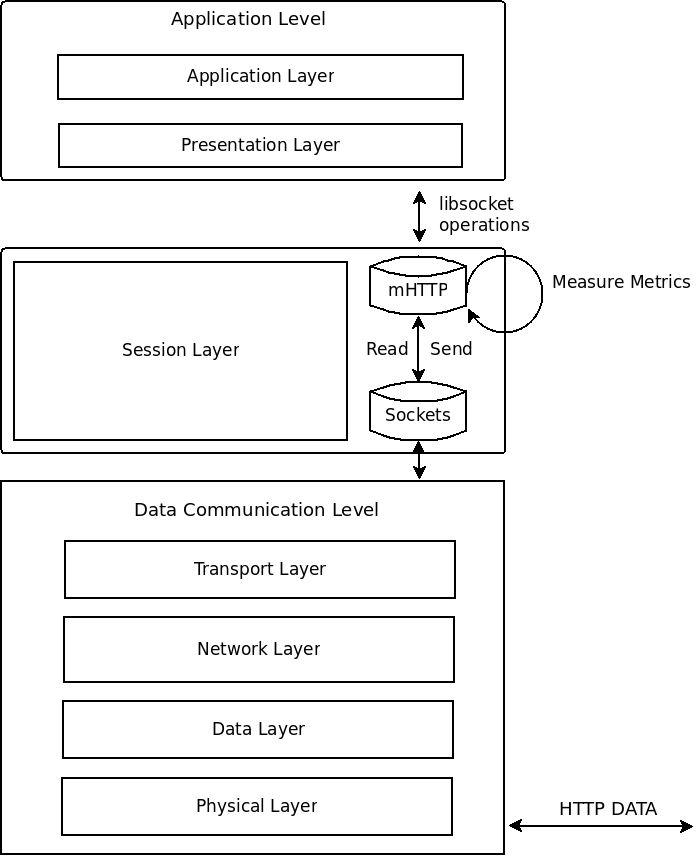
\includegraphics[width=\linewidth]{Figures/mhttp_layer_1}}
%        \end{center}
%        \end{minipage}
%~
        \begin{center}
			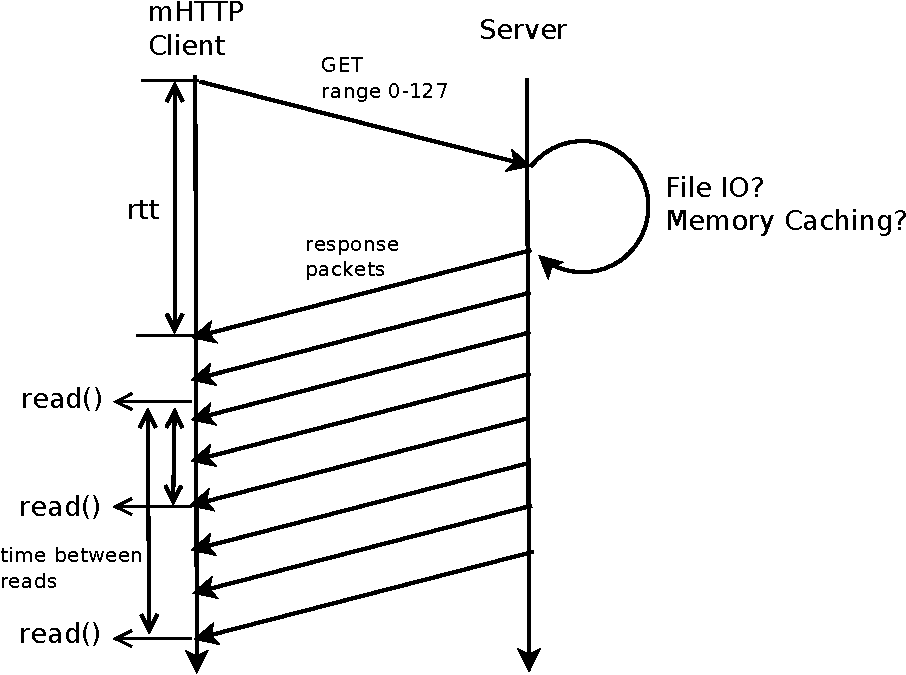
\includegraphics[width=0.7\linewidth]{Figures/scheduler-metrics}
        \end{center}
        \caption{Implications of Request/Response behavior for metrics estimation.}
		\label{fig:metrics}
  \vspace*{-0.3cm}
\end{figure*}

%This means that an event of receiving a byte has to go all the way up from the physical to the application layer which of course adds a certain amount of processing time and falsifies the real physically measured $rtl_i(n)$. 
TCP has a built in retransmission timer which decides when to resend a package after package loss. 
This timer bases its decision on an estimate of $\overline{rtl}_i$ which means that the TCP layer already has its own $\overline{rtl}_i$ estimate and in UNIX systems it is possible to access these values. 
The problem is that these calls are highly platform dependent. 
We try to avoid platform dependency and decide to measure the metrics ourselves inside the \mhttp~library. 
%Further measuring on the session/application layer would give us estimates that are valid on this layer and since our decisions are made for this layer, it is alright to use its estimates.
In order to estimate $rtl_i(n)$ we have to measure the time that goes by between the client sending the first byte of a request to the server and receiving the first byte of the response from the server as we can see in~\fref{fig:metrics}. 
This technique does not take into account the time necessary on the server to process the request until sending the first byte of the response. 
Further, depending on the server hardware and configuration this processing time differs from machine to machine. 
For instance a server that uses resource memory caching will, in most cases have a lower processing time than a server without caching, since reading a resource from disk comes with a huge overhead compared to reading from memory. 
This processing delay is usually comparatively smaller than the link propagation delay. 
%The good news here is that if the server is not overloaded and functioning normally, the processing time should be very small so neglecting it will not harm our estimate badly. 

We send a request to the server for each chunk. 
Directly before sending the request we save a timestamp. 
When the first read operation for the incoming response is performed we take another timestamp and calculate the difference between those two. 
That way we can fairly estimate the time difference between the first byte sent and the first byte received on our layer. 
It follows that during download time we would be able to obtain a new value for $rtl_{i}$ for each chunk request. 
This leads to the question on how to combine these estimates to obtain a more reliable one.
To estimate such a value from a set of samples, rather than simply using the basic mean we could learn from TCP. 
Since a normal mean would give too much importance to extreme values, we should rather consider using a weighed moving average like TCP does~\cite{RFC-6298}. 

On every socket read operation on $c_i$, we measure the current latency 
$rtl_{i}$  and estimate $\overline{rtl}_i$ using a weighed moving average:
$$\overline{rtl}_i = 0.8 \cdot \overline{rtl}_i + 0.2\cdot rtl_{i}.$$

Another issue is the throughput estimate $\overline{R}_i$. 
As we can see in~\fref{fig:metrics} (b) the throughput estimation could be performed by first saving the timestamp of the first socket read event and counting the number of bytes read since then. 
On every further socket read call we divide the total number of bytes since the beginning of the response by the time passed since the first read event. 
That way on every socket read operation (except for the very first one) we estimate single $R_{i}$ values on the \mhttp~layer. 
An important issue we have to consider is that the first read calls might return more bytes in a short amount of time than the following read calls. 
This is due to the fact that we do not measure directly the arrival of the packets on the link, but instead measure when the packets arrive in our \mhttp~layer. 
Until the first bytes are processed and ready for the \mhttp~layer to be read, a lot of bytes might already be buffered in the lower layers. 
This leads to a burst of data in the beginning once all the necessary structures are setup on all the other layers. 
To avoid that this burst falsifies our estimate, we simply neglect the first samples of the first read operations. 

We use the \term{harmonic mean} to estimate the throughput $\overline{R}_i$ on every socket read 
operation. Previous studies have shown that this provides a better throughput estimation
than a moving average estimate and mitigates the impact of large outliers due to 
network variation~\cite{CHEN14-MMA}. Given a series of bandwidth measurements $R_i(t)$, 
where $t=0,1,2,\cdots, n-1$, the \term{harmonic mean} is calculated as:
$$\overline{R}_i = \frac{n+1}{\frac{n}{\overline{R}_i} + \frac{1}{R_i(n+1)}}$$

\section{Path Management}
\label{sec:path-management}

%\begin{figure}[htbp]
%	\centering
%		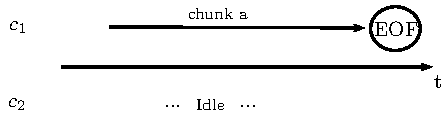
\includegraphics[width=\linewidth]{Figures/path-manager-why-1.pdf}
%		\rule{35em}{0.5pt}
%	\caption[Bad Path Management Scenario]{Bad Path Management: Assuming $c_2$ has a higher throughput than $c_1$, here the better path has idle time due to a bad initial path choice.}
%	\label{fig:bad-path-management-1}
%\end{figure}

The path management determines which end-points to use for a new connection, meaning which client interface and server IP are used to establish a new path. 

In our current approach we define one interface as primary, meaning that this interface will always be used to open the first path to a new server. 
Especially in mobile environments it makes sense to prefer a certain interface such as \wifi, since an \lte~interface might introduce additional economical cost to the user. 

In general, the first request to a new domain is sent over the primary interface and after receiving the response from the server, including the object's actual size, the path manager decides whether it is worth opening a new path. 
In case a second path is needed, we use the second interface to establish a connection. 
Note, that in case of web page downloads most embedded objects are usually downloaded from the same domain. 
Consequently, already opened paths from a previous object download can be reused when requesting another object from the same domain. 
When reusing paths, we always select the in terms of throughput best idle path to start a new request, hence the primary interface might not be chosen first in subsequent requests.

%Further we start work on a second approach we call 2-initial-path mechanism. 
%This mechanism initially and simultaneously opens 2 paths requesting two consecutive chunks of an initial chunk size without knowing the actual file size yet. 
%We expect a great speedup during the initial phase. 
%Still a problem arises if the requested object is of less size than the initial chunk size, meaning that the second request is an out of range request, which will result in an error response by the server. 
%Currently we focus on objects of size bigger than the initial chunk size. 
%Dealing with objects that are smaller than the initial chunk size is part of future work.

\section{Performance Assurance Mechanism}
\label{sec:performance-assurance}

Each scheduling decision is based on an estimated throughput and round-trip-latency value for each active connection. 
It is an issue that these values might change shortly after a scheduling decision was made, since especially in wireless environments link quality changes do frequently occur. 
Taking this into consideration we decide to enhance the \algalpha~and \algslice~algorithm with a lower bound performance assurance mechanism on top, which ensures that the best active path is never idle while a worse performing path is still receiving data. 
This mechanism is only active for the last chunk, since on all previous chunks we can be sure that there is still enough traffic left to distribute among the paths. 
During the download of the last chunk, on each socket read operation the connection compares its estimated download time left with the times other currently open idle paths might need to download the same remaining chunk. 
In case another path might be faster than the current connection plus a certain re-request penalty, we pause the current connection and re-request the missing bytes over the likely faster path.
Since this leads to the case that the slow connection is idle instead, this approach does not directly help us with bundling the throughput of each open path, but it does ensure to at least perform as good as the best established path, thus acting like a lower bound assurance mechanism. 


% implementation chapter
\chapter{Implementation} % Main chapter title
\label{ch:implementation} % Change X to a consecutive number; for referencing this chapter elsewhere, use \ref{ChapterX}

\lhead{Chapter VI. \emph{Implementation}} % Change X to a consecutive number; this is for the header on each page - perhaps a shortened title

The \protoold~prototype could prove the effectiveness of \mhttp~combining the throughput of all interfaces, but still it had a lot of issues and missing features. 
We discuss in detail enhancements and new features of the \protonew~prototype from an engineering point of view. 

\section{General Enhancements}
\label{sec:general-implementation}

In this section we describe the general architecture of the new prototype. 

\begin{figure*}[ht]
		\centering
        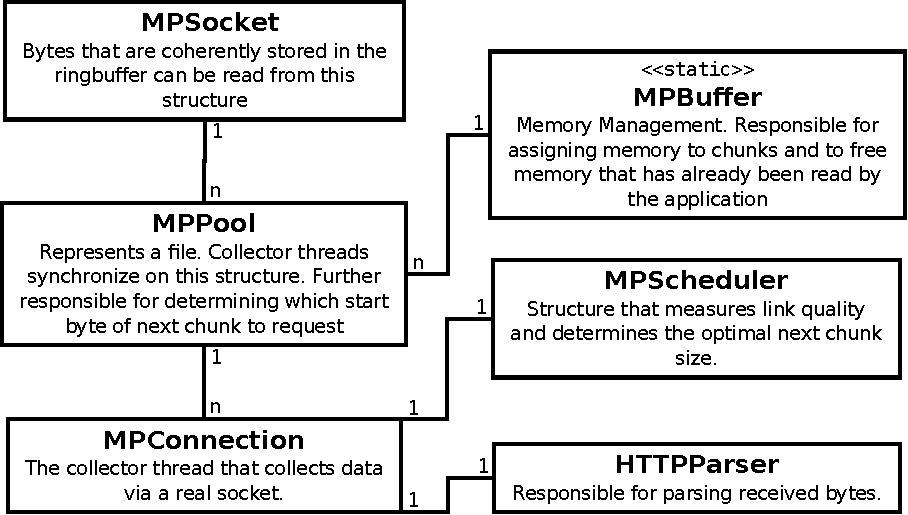
\includegraphics[width=0.7\linewidth]{Figures/implementation-uml.pdf}
        \caption{Illustration of \protonew~object relationships.}
		\label{fig:implementation-uml}
		\vspace*{-0.3cm}
\end{figure*}

In~\fref{fig:implementation-uml} the major objects and their relationships to each other are depicted. 
The \term{MPSocket} object acts as a multipath socket abstraction. 
It provides functions for reading coherently stored bytes via the \term{MPPool} from the \term{MPRingbuffer}. 
The \term{MPPool} object stores information about the running \term{Collector} threads, \ie \term{MPConnection} objects that are responsible for requesting and storing data in the \term{MPBuffer} over a path.
It also keeps track of chunks that still need to be requested and acts as a synchronization point for \term{MPConnection} threads. 
In order to successfully download chunks, each \term{MPConnection} object uses a \term{HTTPParser}, \ie a parser specifically designed and optimized for HTTP traffic, that recognizes different request and response header settings. 
Also, a \term{MPScheduler} object is used to determine the optimal next chunk size for a \term{MPConnection} object. 
Besides determining the optimal chunk size, the \term{MPScheduler} object also estimates the link quality of the path of the designated \term{MPConnection}. 
Through the \term{MPPool}, each \term{MPScheduler} object can make inquiries about the state and performance metrics of other \term{MPConnections}. 
Finally, one static \term{MPBuffer} object is used to manage memory requirements for the dynamic chunks. 

\subsection{New Threading Model}
\label{sec:threading-model}

The \protoold~prototype has exactly one thread that is responsible for sending requests and receiving and processing data from all the open TCP sockets. 
This thread is called \term{Collector} thread. 
Processing data means parsing and copying it into buffers, where the application can later read from. 
While parsing, copying and requesting data the \term{Collector} cannot drain data from any other TCP buffer. 
This behavior bears a potential bottleneck since the TCP buffers might be full before the \term{Collector} has time to drain them, which in return will reduce the TCP receiver window and will force the sender to reduce his sending rate. 
In order to avoid such a scenario it is of utmost importance to ensure that each receiving TCP buffer is drained as fast as possible. 

For that reason we propose a new threading model as illustrated in~\fref{fig:implementation-memory-management}, in which each TCP socket has its own dedicated \term{Collector} thread. 
Creating new threads is relatively expensive in terms of time and resources for the operating system, still this overhead is small compared to the possible gain from a higher parallelization to keep the connections busy and to avoid potential TCP buffer bottlenecks.
To appropriately handle higher parallelization a more sophisticated locking mechanism needs to be applied, which also results in higher overall implementation complexity and when implemented inefficiently might also lead to threads unnecessarily blocking each other which might then result in unnecessary processing overheads. 
To avoid this issue we use the locks only at the beginning of a chunk request. 
At the beginning of a request the thread needs to determine the next request range and allocate memory for the expected data. 
Further, in order to keep track of metrics such as the amount of requests sent, concurrent writes have to be avoided through locking. 
This means that during request preparation there is a chance of threads temporarily blocking each other, but since prior to a request there is no data that needs to be drained from the socket buffer no TCP buffer bottleneck can occur. 
The \term{Collectors} can receive and process data independently from each other, thus avoid an unnecessary blocking bottleneck during those phases. 

\subsection{Reducing System Calls}
\label{sec:system-calls} 

System calls such as memory copies (\eg memcpy) or memory allocations (\eg malloc, mmap) are expensive. 
Especially in case of very short download times, it is important to keep the processing overhead at the client side at a minimum. 
For that reason we change the data flow in \protonew~to reduce memory operations. 

\begin{figure*}[!htb]
		\begin{minipage}[t]{0.8\linewidth}
		\begin{center}
                \subfigure[Data flow in \protoold.]{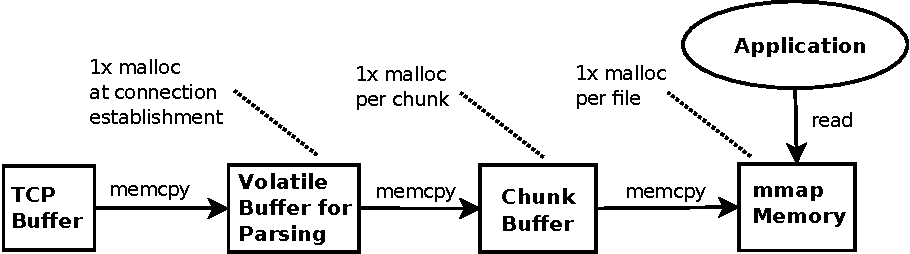
\includegraphics[width=\linewidth]{Figures/implementation-memcpy-old.pdf}}
				\subfigure[Data flow in \protonew.]{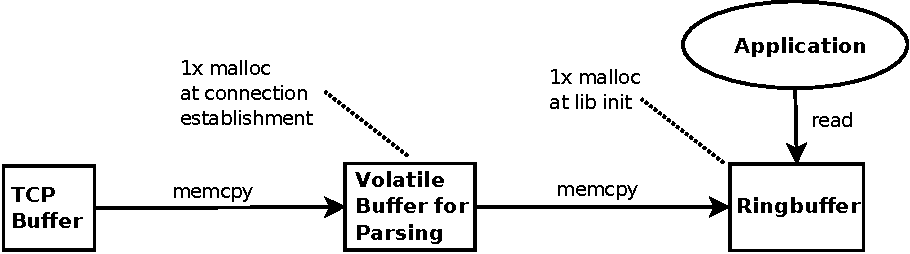
\includegraphics[width=\linewidth]{Figures/implementation-memcpy-new.pdf}}
        \end{center}
        \end{minipage}
		\caption{\label{fig:implementation-memory-flow} Data flow in \protoold~(a) and \protonew~(b).}
\vspace*{-0.3cm}
\end{figure*}

The data flow in \protoold~can be seen in~\fref{fig:implementation-memory-flow} (a). 
For each requested chunk, memory needs to be allocated. 
Note, that chunks might arrive out of order. 
Upon knowing the file size of a web object, \protoold's \term{Collector} allocates the necessary memory for the whole file in assembled state with mmap. 
The \term{Collector} drains data from the TCP buffer into a volatile buffer in which the data is parsed. 
After parsing, the data is copied to its dedicated chunk memory. 
Once two coherent chunks are detected, their data is copied to the mmap allocated file buffer. 
As a result, $3$ memory copies and $1$ memory allocation per chunk plus $1$ memory allocation per file and per established connection are necessary. 

As can be seen in~\fref{fig:implementation-memory-flow} (b), \protonew~does not use a chunk buffer any longer. 
The logical chunk structures reserve memory directly from the ringbuffer instead of allocating their own memory, thus after parsing inside the volatile buffer, data is directly copied to the ringbuffer itself. 
Note, that like in \protoold~chunks can still arrive out-of-order. 
The \term{MPSocket} and \term{MPPool} objects as shown in~\fref{fig:implementation-uml}, are responsible for delivering the data coherently to the application. 
Further, \protonew~only allocates ringbuffer memory once at library initialization time. 
This means, that in total $2$ memory copies per chunk, $1$ memory allocation per established connection and $1$ initial memory allocation at library start time are necessary, thus greatly reducing the amount of system call compared to \protoold. 

Finally, \protonew~also reuses already allocated objects, thus reducing the amount of expensive memory allocations for small objects, \ie \term{MPConnection} and \term{MPPool} objects are all reusable now. 

\subsection{Memory Management}
\label{sec:memory-management}

\protonew~comes with a more advanced memory management than \protoold. 
In \protoold~each chunk needed a memory allocation. 

\begin{figure*}[!htb]
        \begin{minipage}[t]{0.8\linewidth}
		\begin{center}
                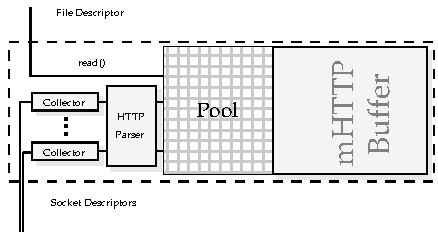
\includegraphics[width=\linewidth]{Figures/design-buffer.pdf}
				\caption{\label{fig:implementation-memory-management}multiHTTP design: I) \mhttp~buffer stores out-of-order received data II) HTTP parser examines and modifies HTTP headers III) collectors gather data from individual TCP connection buffers.}
        \end{center}
        \end{minipage}
  \vspace*{-0.3cm}
\end{figure*}

In contrast, upon initializing the \protonew~library, a simple ringbuffer with a fixed size is created in which data can be stored. 
The application reads directly from the ringbuffer via the \term{MPPool} as shown in~\fref{fig:implementation-memory-management}. 
Instead of allocating new memory each time a chunk of a dynamic size is requested, memory space from the ringbuffer is used, thus saving expensive system calls. 
Moreover, using a ringbuffer allows us to easily keep track of coherently stored bytes. 
Note, that the only requirement for data to be delivered to the application is coherency, meaning that even if a chunk is not completely downloaded, as long as it is coherent, even parts of it can already be read by the application.
This eases the correct delivery of coherent data to the application. 

In this proof-of-concept stage we use wget~\cite{URL-WGET} to download files. 
Since wget does not request files in parallel, but sequentially, a ringbuffer is the easiest, yet efficient choice. 
Note, that in order to work with applications which request files in parallel (such as web browsers like Firefox) another memory management strategy needs to be developed, but that is subject to future \mhttp~implementations. 




\section{Public Website Download}
\label{sec:website-download}

Accessing a web page (\ie a HTML file) typically triggers subsequent downloads
of multiple linked web objects, \eg images (jpg, gif, png), cascading style
sheet (css), and JavaScript (js) files. Thus, we implement a new feature in
\mhttp~that enables the handling of multiple web objects which are subsequently
requested after fetching an HTML page.

Usually, modern GUI web browsers and download managers send HTTP-requests using multiple concurrent processes (multi-threading) in order to better deal with multiple web objects embedded in a single web page. 
Currently, \protonew~does not support parallel file downloads. 
Consequently, objects hosted on the same domain are requested one after another over the same socket abstraction,~\ie the basic operation of wget when \emph{--page-requisites} or \emph{-p} option is set. 
It is important to point out that an HTML page may embed files from different domains, thus the client (wget) establishes several socket abstractions (\ie several mHTTP instances) for accessing a web page. 

\subsection{Static and Dynamic Content}
\label{sec:dynamic-content}

We distinguish between 2 types of content,~\ie static and dynamic. 

\strong{Static content}
It describes files which are not rendered at request time, meaning they already exist on the server before the actual request is sent. 
Dynamic content on the other hand is rendered at request time, meaning the server receives the request and then starts to create the resource. 

Static content can be downloaded by \mhttp, since in most cases it is the same on each server. 
Still, there exist scenarios in which resources differ on different servers. 
For instance when changing a resource on a central server it takes some time until this change reaches every mirror server, so there always is a potential time window in which the servers serve different static content. 
Since this scenario occurs relatively rarely, to save implementation time the new prototype at the current stage does not support this feature yet, but we propose solutions for this issue in~\xref{ch:discussion}, where we talk about content identity verification. 

\strong{Dynamic content} 
This content cannot be downloaded in a multi-request fashion, since it is highly likely that the content differs from source to source. 
Even requests done at different times on the same server can lead to completely different results. 
Since the majority of popular websites contains dynamic content, it is important for \mhttp~to deal with this issue. 
We discovered that it is common for a server to reply with the \emph{Transfer-Encoding: chunked} flag when receiving a byte range request on dynamic content. 
Range requests on static files on the other hand usually do not get a reply with that encoding type, since it does not bring any benefits in that case. 
Chunked encoding is specifically designed for dynamic content. 
It is used to save time by letting the server send parts of the content as soon as they are created and without prior knowledge of the total size of the generated file. 
That way the server does not have to wait for the file to be fully generated and can start sending the already generated parts.
Since the size of a static file is already known upon receiving a request, using cunked encoding here does not bring any benefits. 
For that reason, when receiving such a \emph{Transfer-Encoding: chunked} flag, \mhttp~assumes dynamic content and falls back to using only the initial path and a single request to download the whole resource like normal HTTP would. 
This approach relies on a proper server configuration (\eg not using chunked encoding on static files) and in~\xref{ch:discussion} we will discuss other approaches to identify content identity. 

\subsection{Secure Socket Layer (SSL)}
\label{sec:ssl}

Nowadays privacy concerns are gaining importance. 
This gives rise to a growing number of files delivered via HTTPS,~\ie HTTP over a Secure Socket Layer (SSL). 
The majority of websites among the \emph{Alexa.com} top-1000, currently has at least one file that can only be accessed via HTTPS. 
In order to conduct real-world measurements, \protonew~needs to be able to deal with HTTPS file downloads. 
\protonew~is able to detect HTTPS requests and fall back to a single path download, similar like in~\xref{sec:dynamic-content} when dealing with dynamic content. 
That way we are able to conduct real-world measurements, without the \mhttp~client crashing or getting stuck in the middle. 

Enabling full SSL support means ensuring transparency of \mhttp~to SSL and requires a lot of engineering work. 
This is out of scope of this work and has to be done in future work as discussed in~\xref{ch:discussion}. 

%\section{Scheduler Interface}

\label{sec:scheduler-interface}

In order to easily implement and evaluate different scheduler algorithms we first develope a flexible scheduler interface, meaning a set of hooks that are called on each read and send operation by a collector thread. 

In this section we describe in more detail how the general scheduler call implementation is realized. 

\begin{figure}[htbp]
	\centering
		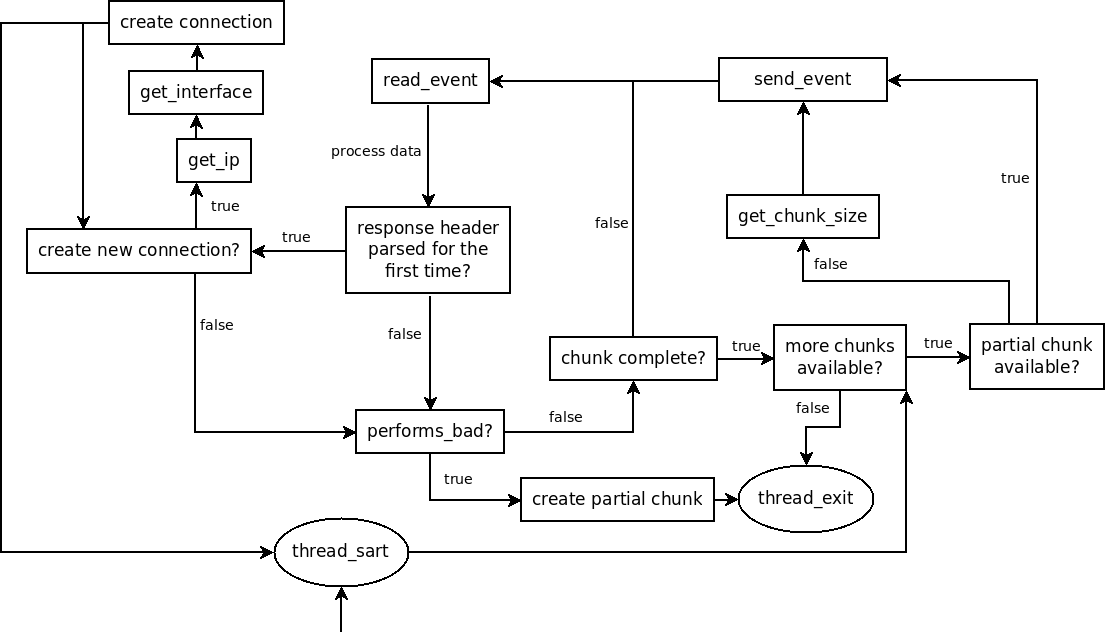
\includegraphics[width=0.48\linewidth]{Figures/scheduler_impl_1}
		\rule{35em}{0.5pt}
	\caption[Collector Thread]{Collector Thread Life Cycle \todo{do in latexdraw}.}
	\label{fig:scheduler_impl_1}
\end{figure}

The scheduler consists of two independent modules. 
First there is the path manager that decides which connection endpoints are chosen to establish a new path. 
Second there is the chunk size scheduler. 
It is making a decision for a request range $s$ for a connection $c$ over interface $i$ at time $j$.

\subsection{Path Manager Calls}
\label{sec:path-manager-calls}

\subsection{Scheduler Calls}
\label{sec:scheduler-calls}

In figure \ref{fig:scheduler_impl_1} the life cycle of a collector thread is depicted. 
A collector thread is responsible for sending requests and receiving the server responses.
During its runtime the thread is doing different calls to the scheduler and path manager interface in order to get instructions on how to behave next. 
By changing the underlying implementations later, we can implement different algorithms without touching the overlaying prototype implementation. 
The thread starts in the chunk management section. 
Here we determine whether or not more chunks need to be requested and what the chunk size is. 

When sending and receiving data the scheduler is notified in order to do proper link measurements. 
Upon receiving data or reaching a certain wait timeout, the thread asks the scheduler whether or not it should shut down due to performance issues. 
This is particularly important in case a path behaves very bad and we need to reschedule the chunk on another link. 
In that case, the already received data of that chunk will be stored and only the missing bytes will be re-requested. 
(TODO: put subsection into fluent text describing the figure)


%\subsection{Hook Set}
%\textbf{Metrics Determination}\newline
%void send\_event(void)\newline
%This hook is called each time prior to a thread making a chunk request. It is used to keep a timestamp to later estimate a rtt sample.\newline\newline

%void read\_event(size\_t bytes)\newline
%This hook is called each time a thread performed a socket read operation. It is used to keep track of the amount of bytes read and timestamps. Further in this function rtt (in case of first response read operation) and throughput $B$ are estimated.\newline\newline

%\textbf{Path Management}\newline
%unsigned long get\_ip()\newline
%This hook is called each time a thread wants to open a new socket. It returns the next suitable server $IP$ for the next path to open, meaning it determines the server endpoint for the next path.\newline\newline

%mpsock\_interface *get\_interface()\newline
%This hook is called each time a thread wants to open a new socket. It returns the interface the client should use for the next path, meaning it determines the client endpoint for the new connection.\newline\newline

%\textbf{Chunk Size}
%size\_t chunk\_size()\newline
%This hook is called each time a thread is preparing a new chunk request. Here is where the main work of the scheduling algorithm is done, since this is where we determine how to chunk our data.\newline\newline

%\textbf{Security Mechanisms}
%int performs\_bad()\newline
%This hook is called each time a thread performed a socket read operation. It determines whether this path is performing bad and whether it should shutdown or stay idle for a while. This is mainly used to avoid scenarios in which a bad performing connection stays busy while another good performing connection stays idle.\newline\newline

%int req\_over\_new\_connection()\newline
%This hook is called each time a thread is forced to stop using its current path. If true, the calling thread will open a new path to request the remaining chunks.


% evaluation chapter
\chapter{Performance Evaluation}
\label{ch:evaluation}

\lhead{Chapter VII. \emph{Performance Evaluation}}

In this chapter we discuss the testbeds and measurements used to evaluate the performance of the different scheduler algorithms. 
Further, we evaluate the achieved results.

\section{Testbed}
\label{sec:evaluation-testbed}



Our evaluation is based on 3 main experiments. 
The first two are single file download evaluations performed in controlled testbeds in Germany and in the US. 
The third is a real-world website download evaluation performed in Germany. 
In this section we describe the testbeds in more detail. 

All experiments are conducted on a Linux client with $2$ network interfaces. 

The download completion time is the major performance metric. 
It is defined as the duration between the first SYN packet from the client and the last data packet from the server. 
Those values can be retrieved by parsing the client \term{tcpdump}~\cite{URL-TCPDUMP} trace files of each download run. 

\strong{German testbed} 
The real-world measurement and one single file download evaluation are conducted in a testbed in a German university campus. 
The client has one \ethernet~and \wifi~network interface. 
Both interfaces are connected to different networks. 
The university campus has a very large data throughput and latency. 
Consequently, in order to evaluate \mhttp~in a more common environment, we throttle the \ethernet~and \wifi~interface to 15Mbps and 10Mbps respectively, for both, the real-world and controlled testbed evaluation. 

We use 2 Debian machines with \term{Apache2}~\cite{URL-APACHE} servers hosting equal copies of the same files. 
%One server is located on the university campus and the other in a German city named Karlsruhe. 
The Apache servers have resource caching enabled, meaning the files are served from memory and do not require relatively expensive disk IO on the servers. 

\begin{figure*}[!htb]
        \begin{minipage}[t]{0.5\linewidth}
		\begin{center}
                \subfigure[Scenario 1 conducted in German testbed.]{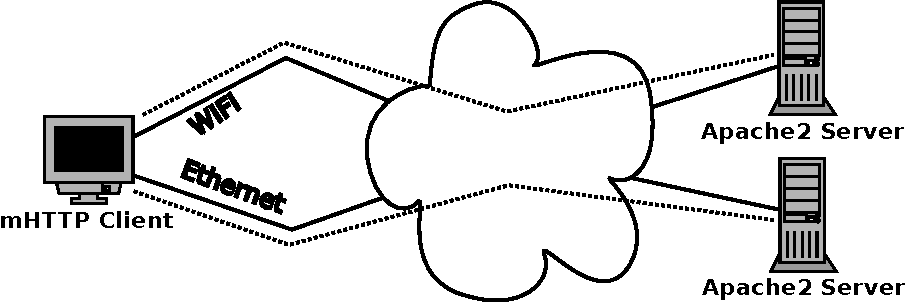
\includegraphics[width=\linewidth]{Figures/evaluation-scenario-1.pdf}}
        \end{center}
        \end{minipage}
~
        \begin{minipage}[t]{0.5\linewidth}
        \begin{center}
                \subfigure[Scenario 2 conducted in US testbed.]{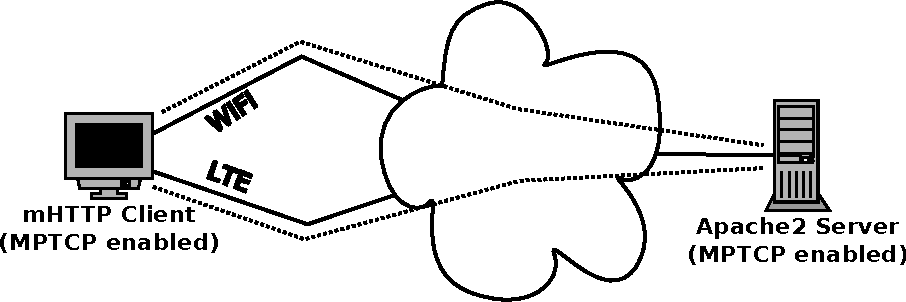
\includegraphics[width=\linewidth]{Figures/evaluation-scenario-2.pdf}}
        \end{center}
        \end{minipage}
        \caption{\label{fig:evaluation-scenarios} Performance evaluation scenario in German testbed (a) and US testbed (b).}
  \vspace*{-0.3cm}
\end{figure*}

For the single file evaluation, inside the German testbed we conduct multi-source tests, meaning both servers are used to concurrently establish connections and download the content, as depicted in~\fref{fig:evaluation-scenarios} (a). 

\strong{US testbed}
In addition to the testbed in Germany, we use an MPTCP enabled testbed in the US \footnote{thanks to Prof. Don Towsley and Dr. Yung-Chih Chen} to get some additional performance data on \mhttp. 
The US testbed is used to compare MPTCP with \mhttp~(with \algslice~scheduling enabled). 
The testbed uses a client with one \wifi~and one \lte~network interface. 
Note, that the MPTCP experiments in this testbed are conducted by our collaborators in the US. 

MPTCP is a single source approach. 
Hence, in order to have a fair comparison, we also use a single server with \mhttp~as depicted in~\fref{fig:evaluation-scenarios} (b). 
Since \mhttp~can freely choose between single- or multi-source downloads, this is not an issue. 
During the experiment, \mhttp~and MPTCP do not interfere with each other, \ie \mhttp~is disabled when MPTCP is running and vice versa. 

\clearpage
\section{Initial Chunk Size}
\label{sec:evaluation-initial-chunk}

\begin{figure*}[!htb]
	\begin{minipage}[t]{0.8\linewidth}
	\begin{center}
      	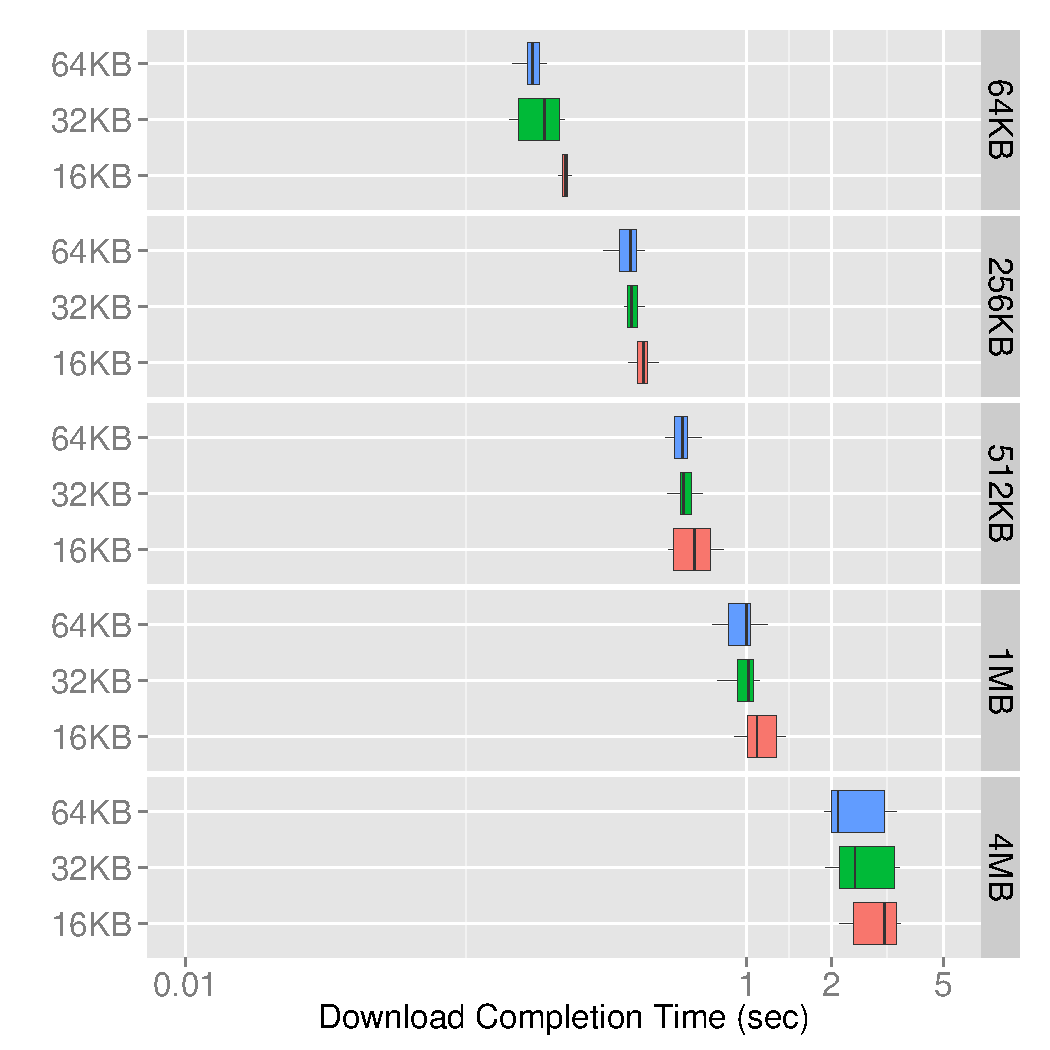
\includegraphics[width=\linewidth]{Figures/dynamic-alpha-initial-chunk.pdf}
		\caption{\label{fig:evaluation-initial-chunk-alpha} Effect of initial chunk size on \algalpha.}
    \end{center}
	\end{minipage}
\vspace*{-0.3cm}
\end{figure*}
\begin{figure*}[!htb]
    \begin{minipage}[t]{0.8\linewidth}
    \begin{center}
        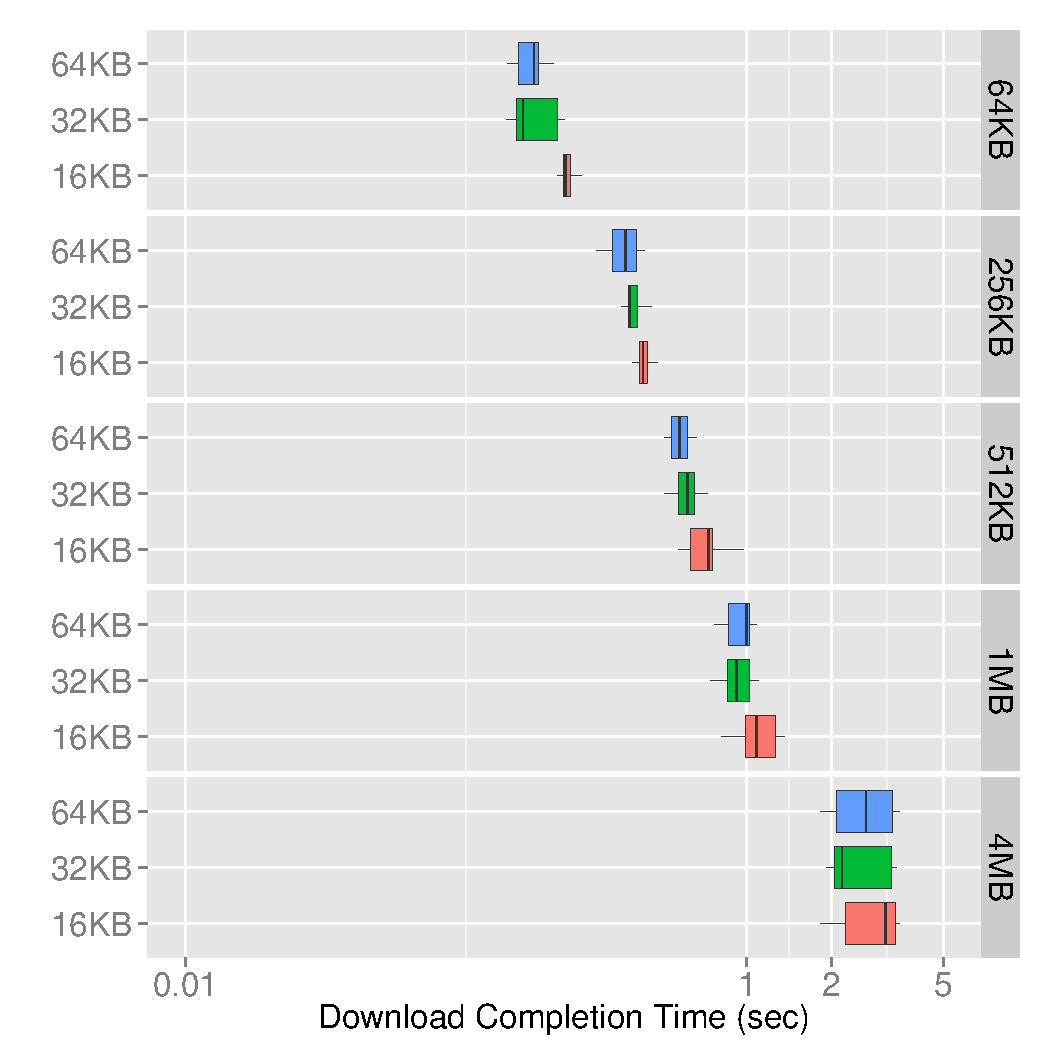
\includegraphics[width=\linewidth]{Figures/dynamic-slice-initial-chunk.pdf}
      	\caption{\label{fig:evaluation-initial-chunk-slice} Effect of initial chunk size on \algslice.}
    \end{center}
    \end{minipage}
  \vspace*{-0.3cm}
\end{figure*}

%- 16KB performs worse, 16KB might not be enough to get a good first link estimate, resulting in small chunks, thus more request overhead

%- 32KB and 64KB seem to perform similar

%- similar results in both schedulers - initial chunk size seems to have same effect

%- be careful in case of website downloads

%- explain that we use 32K initial chunk size (similar like in paper)

We study the effect of the initial chunk size on the \algalpha~and the \algslice~algorithm. 
We take the download completion time as the major metric. 
We measure over $30$ rounds, with each round having a randomized configuration sequence in order to account for traffic dependencies and/or correlation. 
We depict the median, $25-75$\perc percentiles (boxes), and the dispersion (lines, $5-95$\perc percentiles). 
In~\fref{fig:evaluation-initial-chunk-alpha} and~\fref{fig:evaluation-initial-chunk-slice} we see the results for 3 different chunk sizes, \ie $16$KB, $32$KB and $64$KB for \algalpha~and \algslice~respectively. 
The initial chunk size of $16$KB tends to perform worse than initial chunk sizes of $32$KB or $64$KB. 
This is expected; since a small initial chunk could increase the total amount of requests necessary to download a file, which consequently leads to a higher request overhead. 
Moreover, when using very small initial chunks there is a higher chance that the link quality estimate is not very accurate, which might result in bad scheduling decisions for the first chunks. 

We further see that a chunk size of $64$KB tends to perform best, especially on $64$KB files. 
This is reasonable, since the file is downloaded in a single request, whereas with a $32$KB initial chunk a further request is necessary. 
Even when using a second connection, a certain time is necessary to establish that connection. 
This plus the extra request overhead explain the loss compared to $64$KB initial chunks. 

It is important to note that we do not know the link quality prior to an initial chunk request, meaning that in case of a bad link choice a high initial chunk size might be harmful since the initial chunk needs to be downloaded over that link. 
Only after downloading the initial chunk, we obtain information about the link quality to make intelligent chunk size decisions. 
Due to this, we set the initial chunk size to an intermediate value of $32$KB as a compromise between the benefits and the risks. 
Note, that this is an arbitrary choice and further study is necessary to determine the optimal initial chunk size. 

\clearpage
\section{Single File Download Times}
\label{sec:evaluation-single-file}

\begin{figure*}[!htb]
    \begin{minipage}[t]{0.8\linewidth}
	\begin{center}
        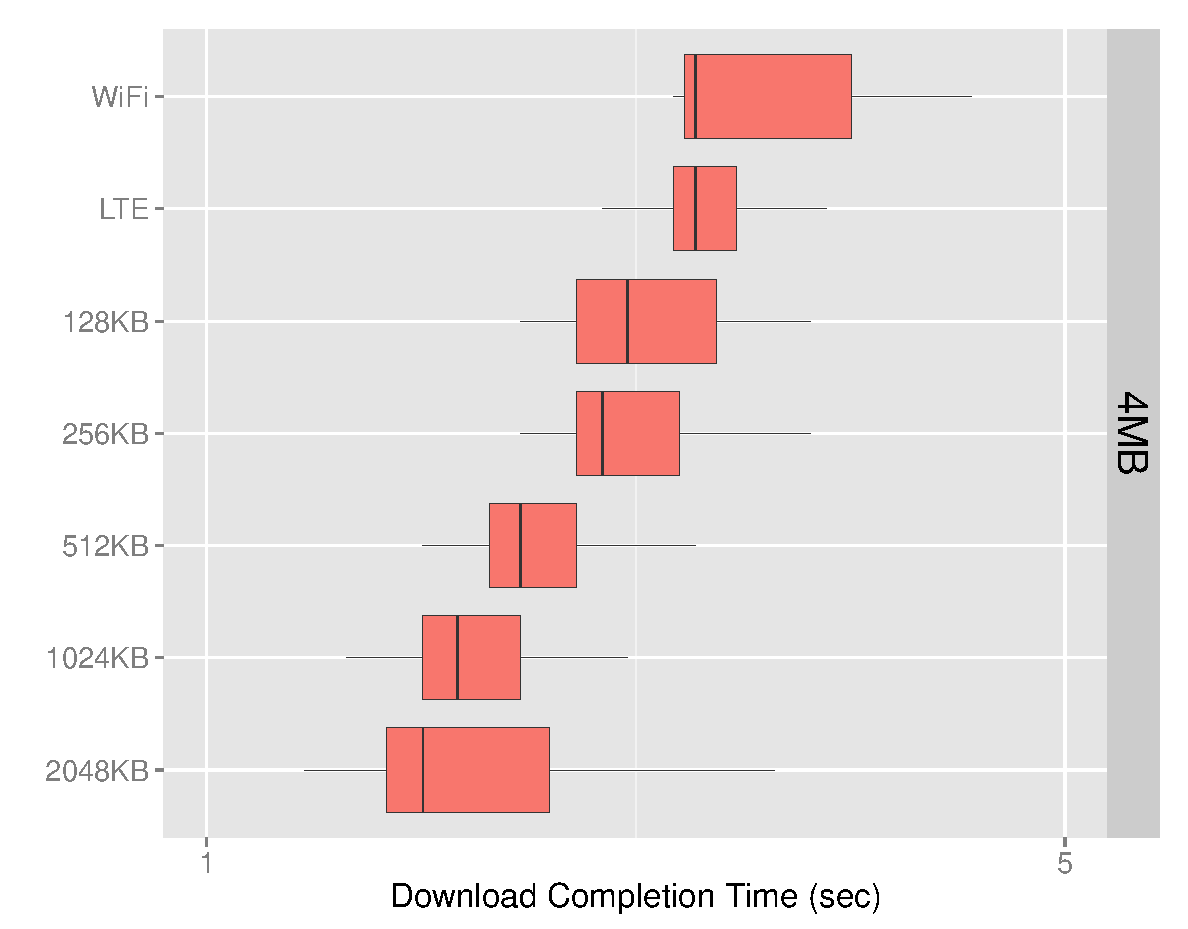
\includegraphics[width=\linewidth]{Figures/baseline-scheduler-us-testbed.pdf}
		\caption{\label{fig:evaluation-baseline-us}\algbase~scheduler results from our US testbed.}
    \end{center}
    \end{minipage}
\vspace*{-0.3cm}
\end{figure*}

We now evaluate the different scheduling approaches for single file downloads, again using the download completion time as the major performance metric. 
We also compare the traffic distributions over the paths. 
In each scenario we measure over $30$ rounds, with each round having a randomized configuration sequence in order to account for traffic dependencies and/or correlation. 
We depict the median, $25-75$\perc percentiles (boxes), and the dispersion (lines, $5-95$\perc percentiles). 
As explained in~\xref{sec:evaluation-initial-chunk}, we use an initial chunk size of $32$KB.

\subsection{Baseline Scheduler}
\label{sec:evaluation-baseline}

In~\fref{fig:evaluation-baseline-us} and~\fref{fig:evaluation-baseline-de} we depict the performance of the \algbase~scheduler of \protoold~as described in~\xref{sec:baseline-scheduler}. 
In~\fref{fig:evaluation-baseline-us} we show the results achieved from our collaborators in the US and in~\fref{fig:evaluation-baseline-de} the results in our testbed in Germany. 
Here, we only illustrate the results of a $4$MB file download, since we only want to emphasize that the optimal fixed chunk size differs from testbed to testbed. 
Deeper studies on the \protoold~\algbase~scheduler for different file sizes have already been performed in the previous research~\cite{KIM13-MHTTP}.

\begin{figure*}[!htb]
    \begin{minipage}[t]{0.8\linewidth}
    \begin{center}
        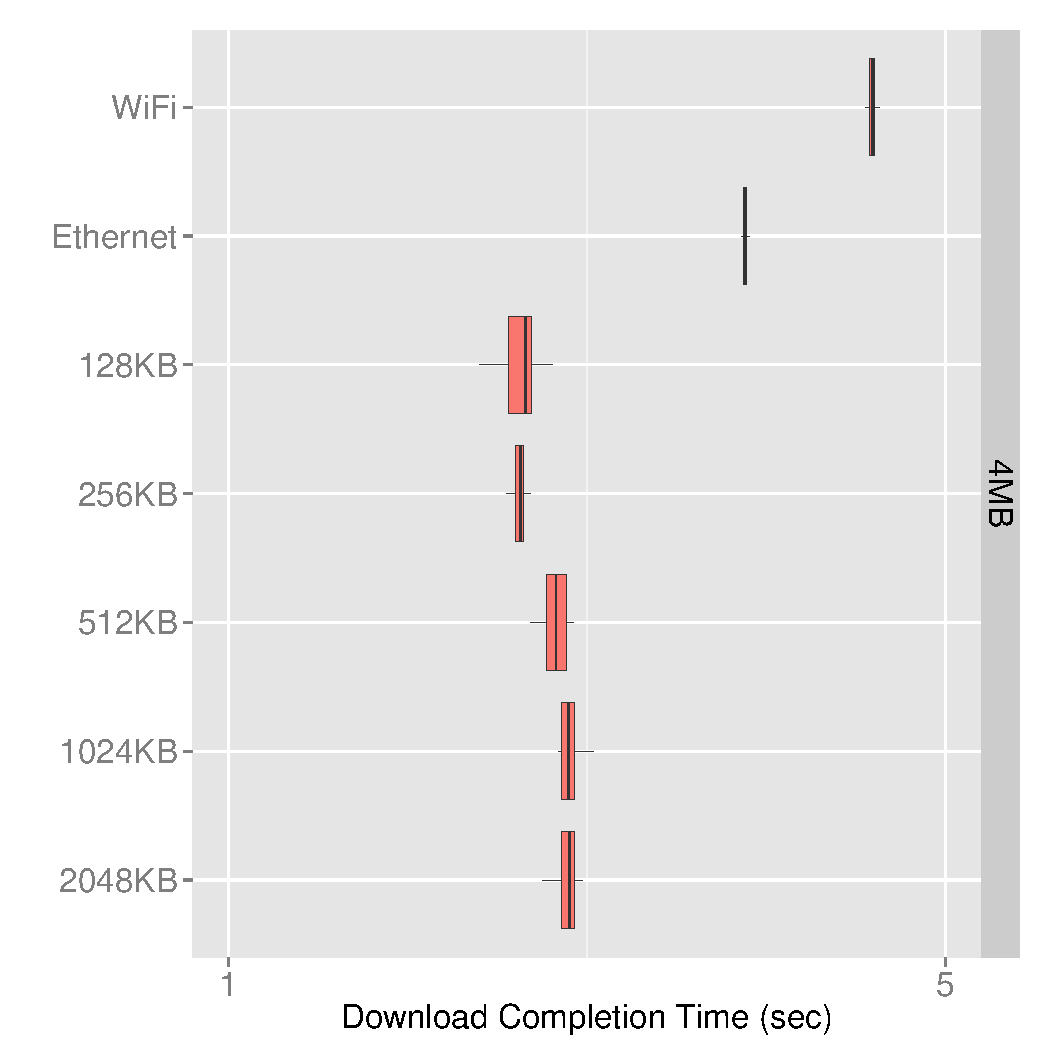
\includegraphics[width=\linewidth]{Figures/baseline-scheduler-de-testbed-4M.pdf}
		\caption{\label{fig:evaluation-baseline-de}\algbase~scheduler results from our German testbed.}
    \end{center}
    \end{minipage}
  \vspace*{-0.3cm}
\end{figure*}

 

In~\fref{fig:evaluation-baseline-us} we can clearly see that the optimal fixed chunk size is $2$MB, whereas in our German testbed in~\fref{fig:evaluation-baseline-de} $128$KB and $256$KB are the optimal fixed chunk sizes. 
When looking at the link qualities in the US testbed, we see that the median throughput is the same. 
An equal distribution of $2$MB chunks on the links performs best, because the request overhead is minimal and both links can more or less handle the same amount of traffic in the same time. 
In contrast to this, we see in our German testbed that both links clearly differ in throughput. 
This proofs that equal traffic distribution might not deliver the optimal result in every case, which is why smaller fixed chunks perform better here, even though they come with a higher request overhead. 

These results perfectly show that the optimal chunk size depends on the link quality and is different from scenario to scenario. 

\pagebreak
\subsection{Implication of $\alpha$ values}
\label{sec:evaluation-alpha}

\begin{figure*}[!htb]
    \begin{minipage}[t]{0.8\linewidth}
	\begin{center}
        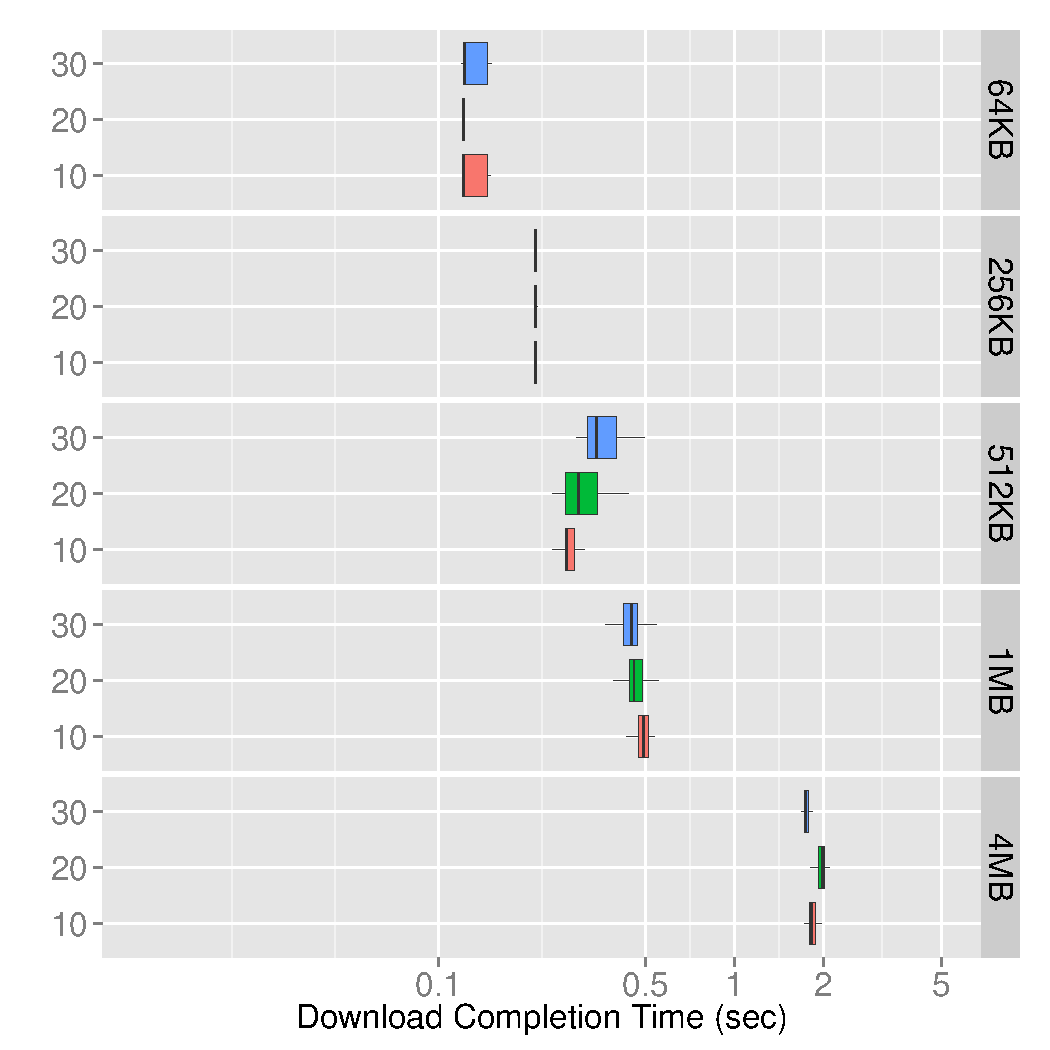
\includegraphics[width=\linewidth]{Figures/dynamic-alpha-alpha.pdf}
		\caption{\label{fig:evaluation-alpha-value-a}Effect of $\alpha_{init}$ in \algalpha~scheduler.}
    \end{center}
    \end{minipage}
\vspace*{-0.3cm}
\end{figure*}

We depict the impact of $\alpha_{init}$ for the \algalpha~scheduler in~\fref{fig:evaluation-alpha-value-a} and the impact of $\alpha_{i,j}$ for the \algslice~scheduler in~\fref{fig:evaluation-alpha-value-b}. 

$\alpha_{init}$ and $\alpha_{i,j}$ are explained in~\xref{sec:alpha-approach} and~\xref{sec:synchronization-approach} respectively. 
In short, a high $\alpha_{init}$ means a high chunk size in the beginning of \algalpha~scheduling and a high $\alpha_{i,j}$ means a high average chunk size during the whole \algslice~scheduling. 

We see that even with changed $\alpha$-values, the performance of the schedulers does not change much. 
On the first view this might be surprising, but can be explained when looking at it closer. 

In case of \algalpha~scheduling, $\alpha_{init}$ merely influences the size of the first chunks. 
Later the chunk size step by step adjusts according to the measured link quality. 
This might be a reason why we do not see a big performance difference between different $\alpha_{init}$ values. 


\begin{figure*}[!htb]
    \begin{minipage}[t]{0.8\linewidth}
    \begin{center}
        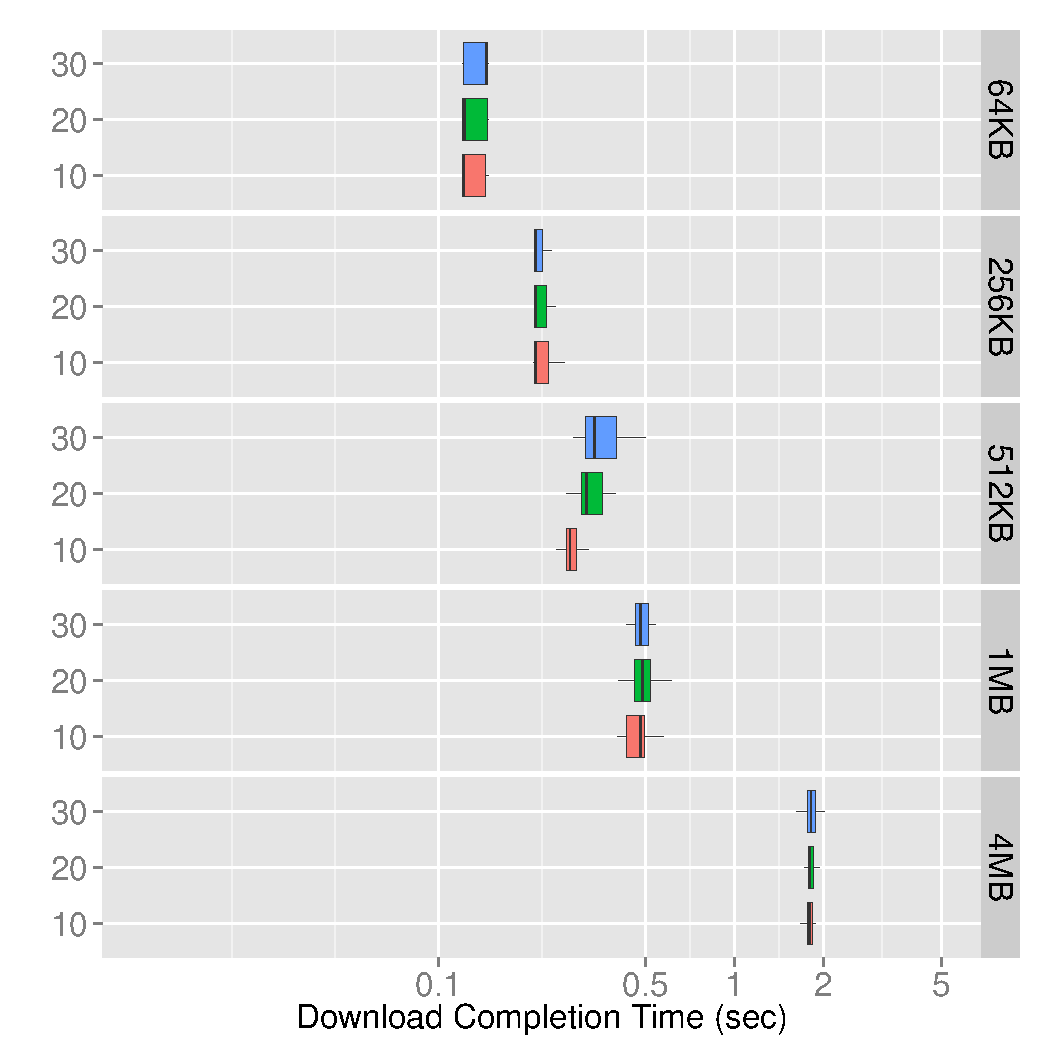
\includegraphics[width=\linewidth]{Figures/dynamic-slice-alpha.pdf}
		\caption{\label{fig:evaluation-alpha-value-b}Effect of $\alpha_{i,j}$ in \algslice~scheduler.}
    \end{center}
    \end{minipage}
  \vspace*{-0.3cm}
\end{figure*}

For \algslice~scheduling, a bigger $\alpha_{i,j}$, means larger chunks in the middle of the download, which consequently also means less overall request overhead. 
In our testbed, bigger $\alpha_{i,j}$ do not make a big difference though. 

To summarize, a high $\alpha_{init}$ might reduce the request overhead in the beginning, but it comes with the risk that we lose adaptiveness to link quality changes. 
This is why from now on we use the intermediate value $\alpha_{init} = 20$ for our further measurements. 
Similarly for $\alpha_{i,j}$, where a high value might reduce request overhead for the loss of link adaptiveness, we also decide to use from now on the intermediate value $\alpha_{i,j} = 20$. 

\pagebreak
\subsection{Comparison of different Schedulers} 
\label{sec:evaluation-schedulers-mixed}

\begin{figure*}[!htb]
    \begin{minipage}[t]{0.8\linewidth}
	\begin{center}
        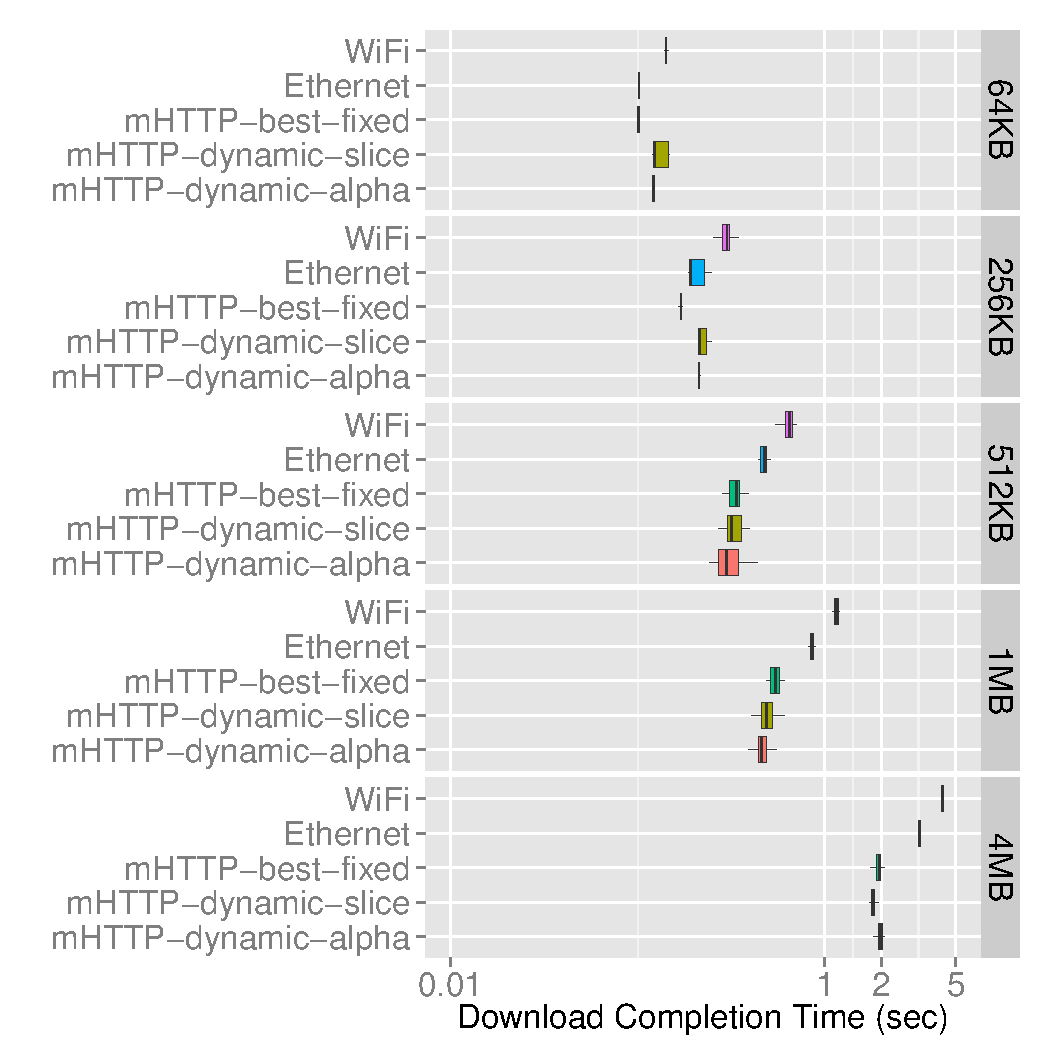
\includegraphics[width=\linewidth]{Figures/scheduler-comparison.pdf}
		\caption{\label{fig:evaluation-comparison-times}Download times of different scheduler algorithms.}
    \end{center}
    \end{minipage}
\vspace*{-0.3cm}
\end{figure*}

In~\fref{fig:evaluation-comparison-times} we depict the download times of different files for each scheduler, \ie \algalpha~(dynamic-alpha), \algslice~(dynamic-slice) and the \algbase~scheduler (best-fixed). 
Also, we show the download times of each single interface, \ie \ethernet~and \wifi.
$\alpha_{init}$ and $\alpha_{i,j}$ are both set to $20$, as previously explained in~\xref{sec:evaluation-alpha}. 
Further, as discussed in~\xref{sec:evaluation-initial-chunk}, the initial chunk size is set to $32$KB.
Please note that the depicted results of the \algbase~scheduler are the best performing fixed chunk sizes for our testbed, meaning all other fixed chunk sizes performed worse than these results. 
We can see that on small files, such as $64-256$KB, our developed schedulers perform nearly as good as the best fixed chunk size. 
The slight difference between them can be explained through the extra request overhead, since our new schedulers tend to perform more requests on small files due to the small initial chunk size. 
Starting from $512$KB our new schedulers even tend to perform slightly better than the best fixed chunk size. 


\begin{figure*}[!htb]
    \begin{minipage}[t]{0.8\linewidth}
    \begin{center}
        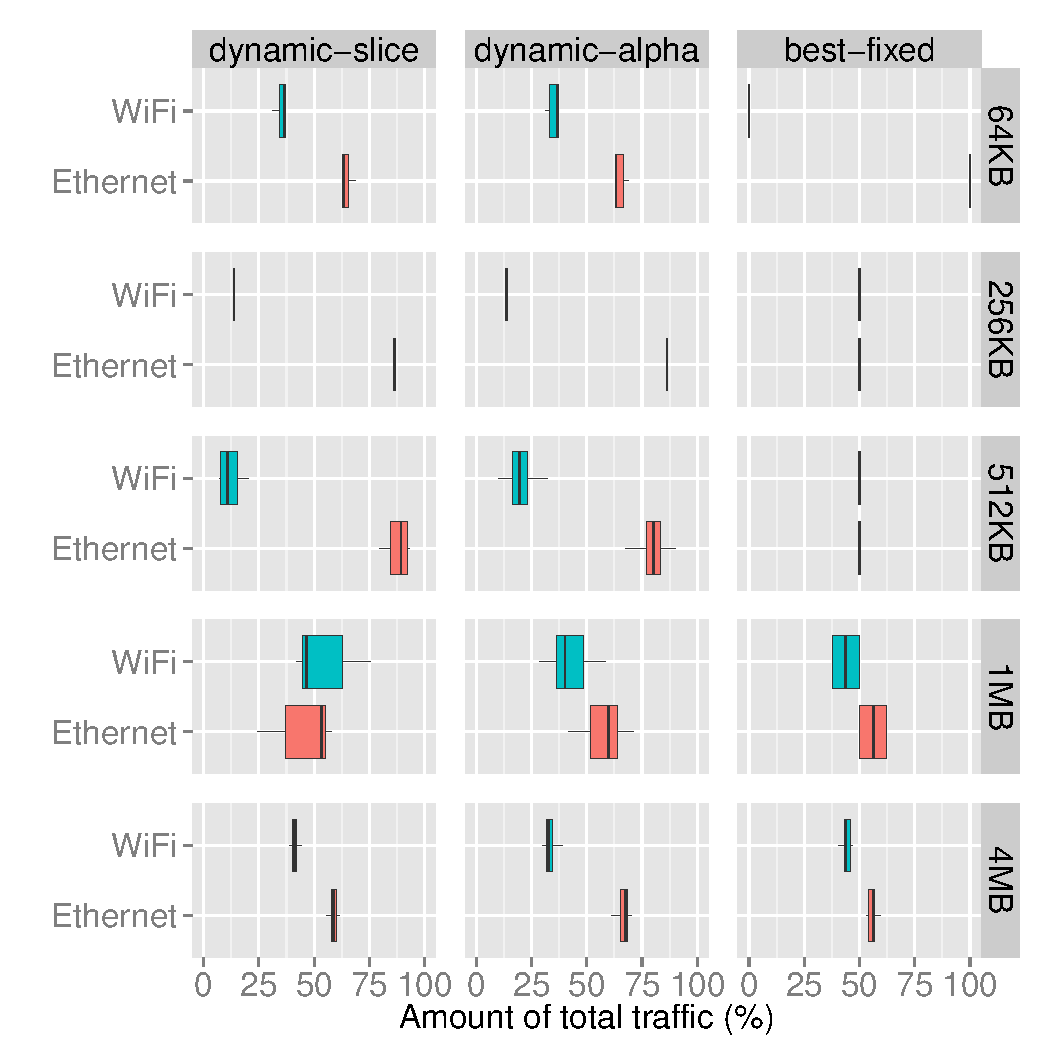
\includegraphics[width=\linewidth]{Figures/traffic-distribution-all.pdf}
		\caption{\label{fig:evaluation-comparison-traffic}Traffic distributions among the paths.}
    \end{center}
    \end{minipage}
  \vspace*{-0.3cm}
\end{figure*}

When looking at the traffic distribution among the paths, as depicted in~\fref{fig:evaluation-comparison-traffic}, we see that the fixed chunk size scheduler tends to distribute the traffic equally, whereas our new developed schedulers distribute the traffic according to the links' qualities. 
Especially in case of $256$KB and $512$KB file downloads, we can see that the fixed chunk scheduler does not take link qualities into account and distributes the chunks evenly over the paths. 
In case of the $64$KB file download, the fixed chunk size is big enough to download the whole file in one chunk, resulting in the whole traffic being processed over the \ethernet~link, while the \wifi~link stays idle. 
In the traffic distribution for $1$MB file downloads with the \algslice~scheduler, we see that in a few scenarios more traffic has been scheduled over the supposedly weaker interface, \ie~the \wifi~interface. 
It is hard to find the exact reason for this behavior, but since the download time in this case is similar to the one with the \algalpha~scheduler, we see that the scheduler made the correct choices at that time. 

Overall the \algalpha~and the \algslice~scheduler perform very similar, in both traffic distribution and download time. 
One reason for this might be, that the \algslice~scheduler tends to have smaller chunks towards the end of the download. 
The gain attained from the synchronization might get neglected due to this extra request overhead. 

Even though in this experiment both advanced schedulers behave similar, we expect the \algslice~scheduler to be superior in very unstable mobile environments. 
Note, that the links in our German testbed have a relatively stable performance. 
We expect the \algslice~scheduler to behave better in very unstable environments, since it takes an extra constraint into account, \ie the assumption that both connections should finish downloading their last chunk at the same time.
In~\chref{ch:discussion} we talk about future mobility studies, in which we expect the \algslice~algorithm to perform better than the \algalpha~scheduler. 
In the following evaluations we use the \algslice~scheduler as \mhttp's default scheduler. 

\subsection{mHTTP vs. MPTCP}
\label{sec:evaluation-mptcp}

\begin{figure*}[!htb]
    \begin{minipage}[t]{0.8\linewidth}
	\begin{center}
        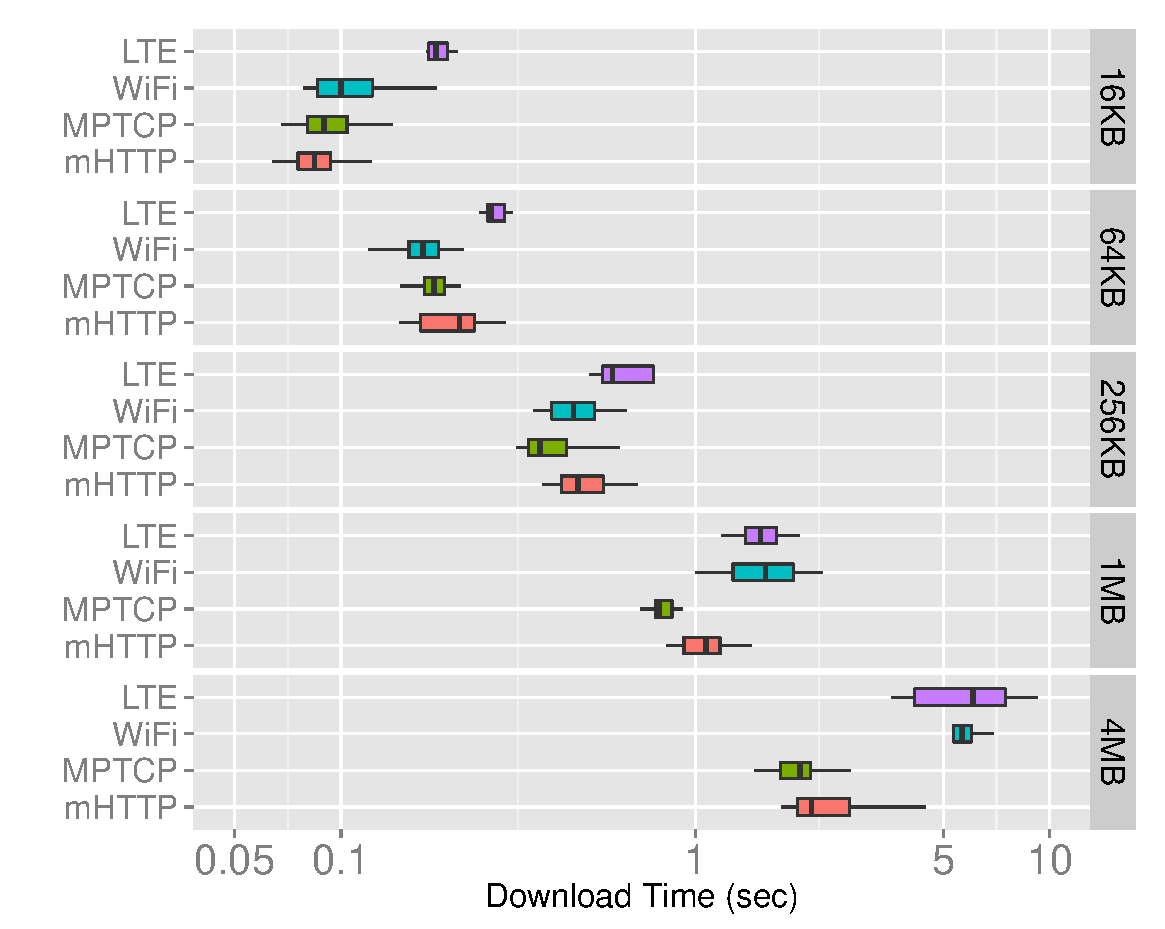
\includegraphics[width=\linewidth]{Figures/umass-mhttp-mptcp-stcp-32k.pdf}
		\caption{\label{fig:evaluation-mptcp-times}Download times of \mhttp~vs. MPTCP vs. HTTP.}
    \end{center}
    \end{minipage}
\vspace*{-0.3cm}
\end{figure*}

We use the \algslice~scheduler to compare \mhttp~with MPTCP, due to the reasons explained in~\xref{sec:evaluation-schedulers-mixed}.
$\alpha_{init}$ and $\alpha_{i,j}$ are both set to $20$, as previously explained in~\xref{sec:evaluation-alpha}. 
Further, as discussed in~\xref{sec:evaluation-initial-chunk}, the initial chunk size is set to $32$KB.
For the experiment we use our US testbed as explained in~\xref{sec:evaluation-testbed}. 

\begin{figure*}[!htb]
    \begin{minipage}[t]{0.8\linewidth}
    \begin{center}
        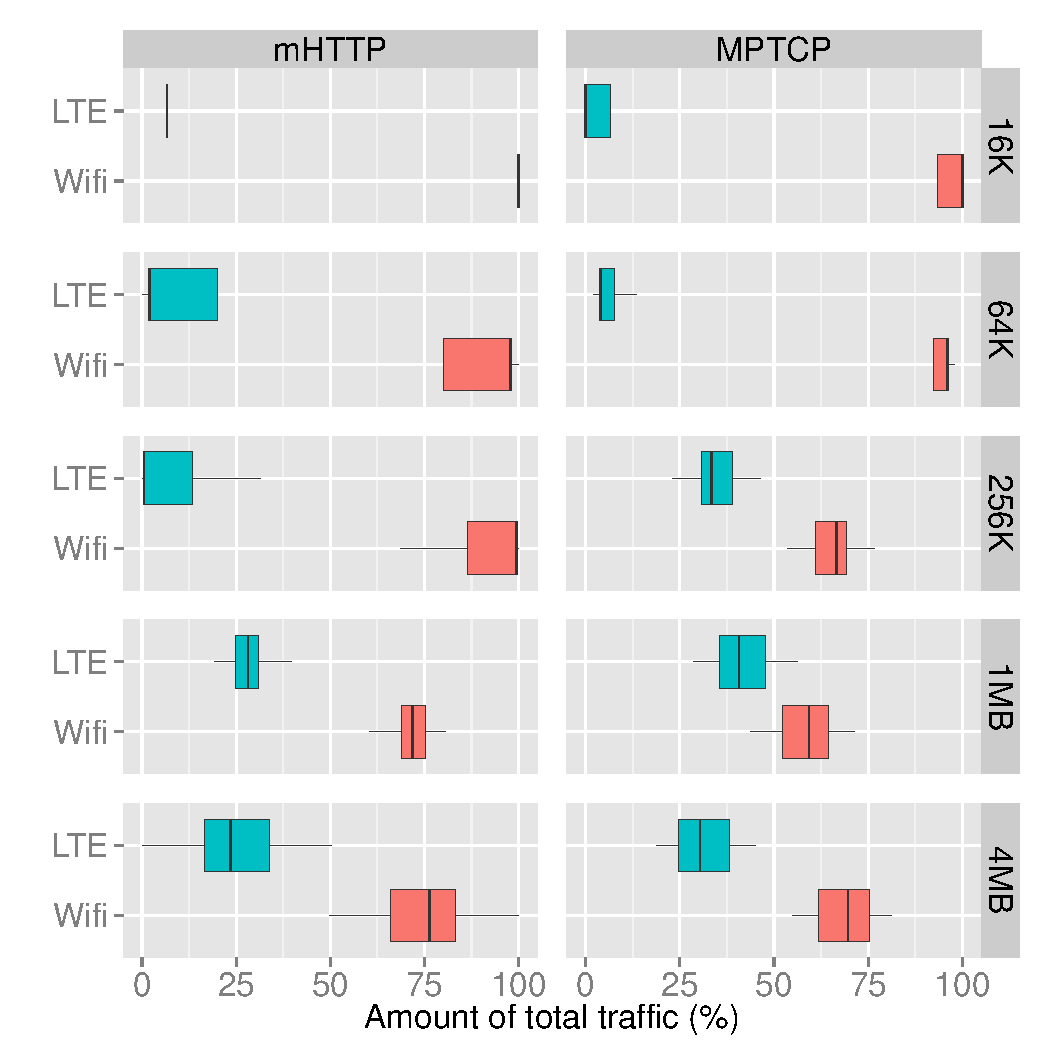
\includegraphics[width=\linewidth]{Figures/umass-mhttp-mptcp-stcp-fraction.pdf}
		\caption{\label{fig:evaluation-mptcp-traffic}Traffic distribution of \mhttp~vs. MPTCP.}
    \end{center}
    \end{minipage}
  \vspace*{-0.3cm}
\end{figure*}

The results of the download times are shown in~\fref{fig:evaluation-mptcp-times}. 
We see that MPTCP performs slightly better than \mhttp~with \algslice~scheduling. 
However, the difference between both is small, especially in the $4$MB download case. 
It is important to mention, that our US testbed is optimized for MPTCP beyond the default MPTCP standard. 
The proposed standard uses coupled congestion control~\cite{RFC-6356}, whereas our testbed uses uncoupled congestion control with Cubic~\cite{TCP-CUBIC}, meaning that in the standard case MPTCP would likely perform worse than what we observe here \cite{CHEN13-MSM}. 

In~\fref{fig:evaluation-mptcp-traffic}, we illustrate the traffic distribution of \mhttp~and MPTCP over the available network interfaces. 
We see that MPTCP transmits a larger fraction of traffic over the \lte~interface, especially in case of small files (\eg $256$KB). 
This might explain, why MPTCP performs slightly better here. 
For $4$MB files, the difference in traffic distribution is negligible. 

\pagebreak

\clearpage
\section{Website Downloads}
\label{sec:evaluation-website}

\begin{figure*}[!htb]
    \begin{minipage}[t]{0.8\linewidth}
	\begin{center}
        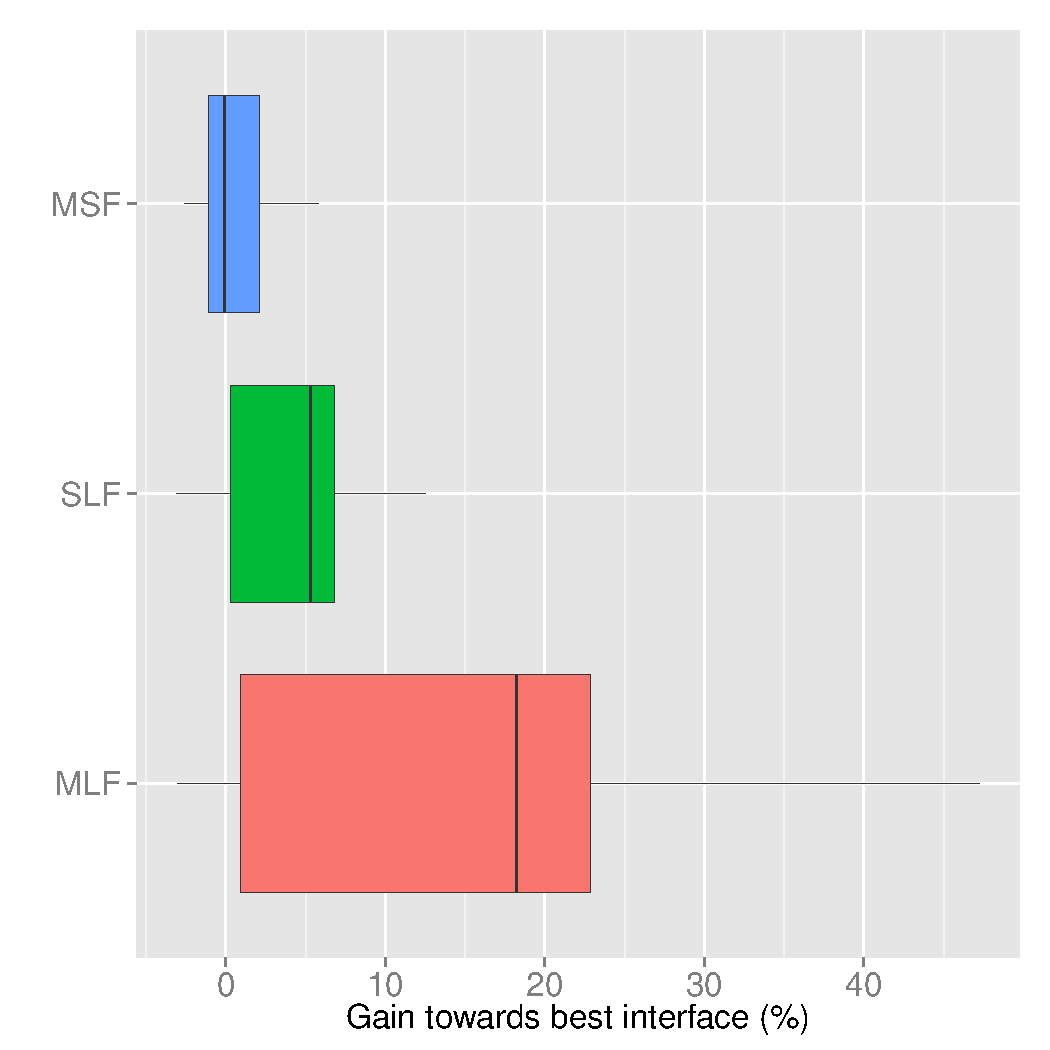
\includegraphics[width=\linewidth]{Figures/website-category-performance.pdf}
		\caption{\label{fig:website-performance-category}Performance gain (\perc) of each category towards best interface (\ethernet).}
    \end{center}
    \end{minipage}
\vspace*{-0.3cm}
\end{figure*}

Web pages differ in number and size of embedded files. 
\mhttp~is specifically designed for large files. 
Therefore, its general performance on websites is highly dependent on the portion of large embedded files. 
For a proper evaluation we select 24 web pages from \term{Alexa.com}~\cite{URL-ALEXA} and divide them into 3 categories. 
Each category is then evaluated separately, in order to study the effect of \mhttp~on different kinds of websites. 
As listed in~\tref{tab:website-category}, the categories are many small files (\term{MSF}), some large files (\term{SLF}) and 
many large files (\term{MLF}). 
The categorization is mainly based on the fraction of large files ($>$1MB) embedded in the page. 

%The performance of downloading web pages using \mhttp is significantly affected 
%by the size and number of embedded files. Therefore, the performance evaluation of
%\mhttp on random web pages cannot be seen as the general result. 
%Consequently, we divide web pages into three different categories according to the size 
%of the embedded objects and evaluate \mhttp over each category separately. The three 
%categories are many small files (\term{MSF}), some large
%files (\term{SLF}), and many large files (\term{MLF}). The categorization is mainly based on
%the fraction of large files ($>$1MB) embedded in the page. The categorization
%scheme and the number of samples are listed in~\tref{tab:website-category}.

A web page has to meet certain requirements in order to be used for our experiments.  
First, the content of a web page should not change too
frequently since our measurement is performed repeatedly in different time
periods. Second, the majority of embedded objects in the web page should not be
dynamically generated on every access request. Third, the majority of web
objects on the web server must be accessible through HTTP,~\ie no HTTPS-only
servers, without authentication. All 24 selected web pages fulfill these criteria. 
Note, that for this experiment all selected web pages are index pages. 
Index pages tend to have smaller embedded objects that can be quickly delivered to the user. 

%For our experiments, these pages are manually verified and selected to meet
%certain requirements. First, the content of a web page should not change too
%frequently since our measurement is performed repeatedly in different time
%periods. Second, the majority of embedded objects in the web page should not be
%dynamically generated on every access request. Third, the majority of web
%objects on the web server must be accessible through HTTP,~\ie no HTTPS-only
%servers, without authentication. As a result, we select 24 web pages in
%total.

\begin{figure*}[!htb]
    \begin{minipage}[t]{0.8\linewidth}
    \begin{center}
        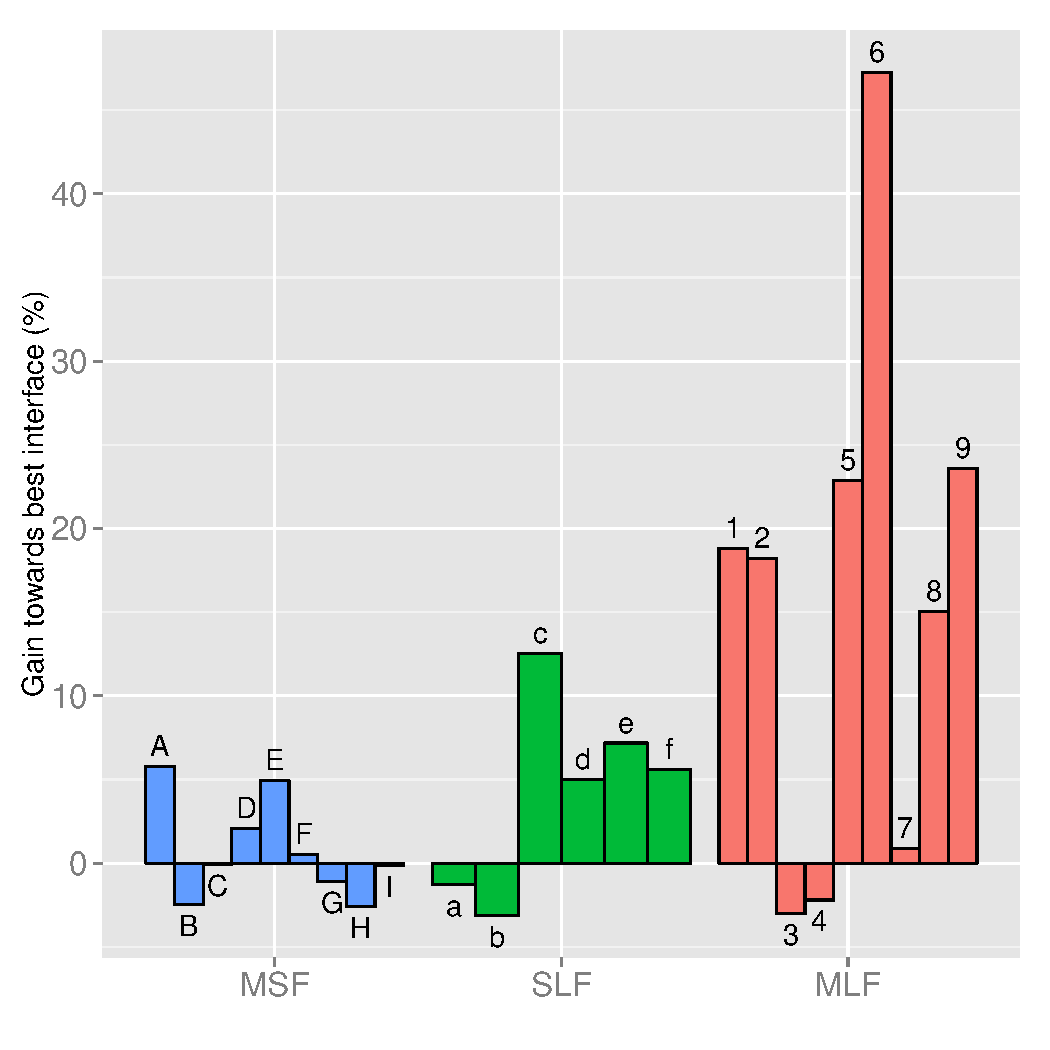
\includegraphics[width=\linewidth]{Figures/website-individual-performance.pdf}
		\caption{\label{fig:website-performance-site}Performance gain (\perc) of each website towards best interface (\ethernet).}
    \end{center}
    \end{minipage}
  \vspace*{-0.3cm}
\end{figure*}

Our previous experiments were conducted in controlled testbeds in Germany and in the US. 
For the web performance experiment we use a laptop equipped with an \ethernet~interface and a \wifi~interface, both connected to the Internet via two different access networks. 
The laptop is located in a German university campus. 
Similar like with our controlled German testbed, we throttle the \ethernet~and \wifi~interface to 15Mbps and 10Mbps respectively, in order to simulate a more common environment. 
We use \mhttp~with an initial chunk size of $32$KB and the \algslice~scheduler, due to the reasons explained in~\xref{sec:evaluation-schedulers-mixed} and~\xref{sec:evaluation-initial-chunk}.
$\alpha_{i,j}$ is set to $20$, as explained in~\xref{sec:evaluation-alpha}.

%Unlike our previous experiments that were performed in controlled testbeds in Germany and in the US, the
%web workload experiment is conducted in a German university campus using a
%laptop equipped with an \ethernet~interface and a \wifi~interface connected to
%the Internet via two different access networks. We use \mhttp~with
%an initial chunk size of $32$KB and the \algslice~scheduler, due to reasons explained in~\xref{sec:evaluation-schedulers-mixed} and~\xref{sec:evaluation-initial-chunk}.
%$\alpha_{i,j}$ is set to $20$, as explained in~\xref{sec:evaluation-alpha}.

\fref{fig:website-performance-category} and~\fref{fig:website-performance-site} illustrate the performance gain and
loss of \mhttp~in web page downloads compared to HTTP over the best performing
interface (\ethernet~in our experiment).
As expected, we observe essentially no gain for the \term{MSF} category. 
This category has no large files embedded, which is why this result is not surprising. 
The \term{SLF} and \term{MLF} category web sites on the other hand gain around $5$\perc and $18$\perc respectively. 

%\fref{fig:website-performance} (a) and (b) illustrate the performance gain and
%loss of \mhttp~in web page downloads compared to HTTP over the best performing
%interface (\ethernet~in our experiment). From the results we observe that 
%there is essentially no gain for websites in the \term{MSF} category, a gain of around $5$\perc for 
%those in the \term{SLF} category, and around $18$\perc for websites in the \term{MLF} category. The lack of 
%a performance gain for the \term{MSF} category is not surprising since web pages that belong 
%to this category do not embed any large files. 

\fref{fig:website-performance-site} depicts the performance gain achieved for each individual 
website in each category. The web page, alias \emph{A} in the \term{MSF}
category in~\fref{fig:website-performance-site} shows good performance even without
any large files. On closer investigation, we find that the web
page embeds many files that are smaller than $1$MB, but much larger than the
initial chunk size. 

\begin{table}[!htb]
\begin{center}
\tabcolsep3mm
\begin{tabular*}{0.98\linewidth}{lrrr}
\toprule
                                             & \scriptsize{\term{MSF}}      & \scriptsize{\term{SLF}}                & \scriptsize{\term{MLF}}  \\
\midrule
\scriptsize{\perc of large files ($>$ 1 MB)} & \scriptsize{0\perc}   & \scriptsize{$<$ 1\perc}         & \scriptsize{$>$ 1\perc} \\
\scriptsize{Median(\perc of large files)}    & \scriptsize{0\perc}   & \scriptsize{$0.59$\perc}  & \scriptsize{$2.5$\perc} \\
\scriptsize{No. of samples (pages)}          & \scriptsize{9} & \scriptsize{6}           & \scriptsize{9}        \\
%\multicolumn{4}{l}{}\\
\bottomrule
\end{tabular*}
\end{center}
\caption{Web page categorization scheme}
\label{tab:website-category}
\vspace{-3mm}
\end{table}

For websites in the \term{SLF} and \term{MLF} categories, we observe a significant performance 
gain using \mhttp. 
This is especially true for the \term{SLF} category where the fraction of large files is less than $1$\perc. 
Here, one of the web pages (\emph{c} in~\fref{fig:website-performance-site}) shows more than $10$\perc gain using \mhttp. 
Considering the small difference between the percentage of large files in \term{SLF} (median $0.59$\perc) and in \term{MLF} (median $2.5$\perc), the difference in the median gain between the two categories is significantly high. 
In particular, web page \emph{6} embeds around $2.5$\perc of large files and has a median file size of around $170$KB and exhibits almost $50$\perc of the performance gain by using \mhttp.
This shows that \mhttp~does not harm the browsing of web pages with no large files, but it has the potential to greatly decrease the download times of web sites with large embedded ones and already a small fraction of large embedded objects is sufficient, to witness a gain. 

%This shows again the well-known fact that while there may be many small files, 
%large files are responsible for the bulk of the total value traffic in the Internet.
%Hence, multipath approaches such as \mhttp~can bring significant decreases 
%in download times to users.


% discussion / future work
\chapter{Discussion \& Future Work}
\label{ch:discussion}

\lhead{Chapter IIX. \emph{Discussion \& Future Work}} % Change X to a consecutive number; this is for the header on each page - perhaps a shortened title

%- pipelining

%- E-tag

%- proper SSL support -- enable SPDY

In this chapter we discuss the current limitations of \protonew~and how we intent to solve them in the future. 

\strong{Verification of the content identity} 
As discussed in~\xref{sec:dynamic-content}, due to the locale or time difference it is possible that the same static content differs on different servers in a certain time window. 
Further, relying on the \emph{Transfer-Encoding: chunked} flag to detect dynamic content can lead to failures, since it depends on a proper server configuration. 
In such scenarios \mhttp~needs to fall back to normal HTTP in order to avoid corrupting the resource for the application. 
We propose two solutions to identify such scenarios. 
First, through requesting a few more bytes in the initial request, we can then compare the redundantly received extra bytes with the first few bytes of the first chunk of the second connection. 
In case they differ, we know that the resources are not the same and fall back to normal HTTP. 
Obviously the drawback of this method would be that the initial chunk downloads a few redundant bytes, which could be accounted as extra overhead. 
It is object of future research how many extra bytes would be necessary to make a fair decision on resource equality and how much they harm the overall download speed. 
Second, we could use HTTP's Entity Tag (\term{ETag}~\cite{RFC-2616}). 
The \term{ETag} is a hash value of the resource, thus could be used to detect mismatches. 
Of course, in order to use it, the \term{ETag} functionality needs to be enabled by the server. 

\strong{More Transparency towards the application layer} 
Currently \mhttp~only supports a minimal set of socket API functions to prove its core concept with the wget application. 
In the future we want to expand this set of functions supported by \mhttp, to support calls from modern browsers such as FireFox or Chrome. 
This would enable \mhttp~to be evaluated with concurrent resource requests or pipelining functionalities applied in modern browsers. 

\strong{SSL support}
As already mentioned in~\xref{sec:ssl}, a growing number of files is only accessible via HTTPS, because of growing privacy and security concerns. 
\protonew~can detect HTTPS requests and download them through a single path, thus losing the benefit of the multi-path approach. 
It is of utmost importance to implement a transparent channel between SSL and \mhttp, in order to enable \mhttp~to download HTTPS resources in a multi-path fashion. 

\strong{Comparison with similar technologies}
Many different multi-path technologies already exist with different traffic scheduling approaches. 
In this work we only compare the performance of our best scheduler, \ie \algslice~with the performance of MPTCP. 
Setting up a testbed to compare \mhttp~with other technologies such as Google's SPDY protocol~\cite{BELSHE12-SPDY} is a task for future studies. 

\strong{Mobility study}
In this work, the evaluation was done in relatively stable and static environments, \ie a non moving client with $2$ interfaces with stable internet connections. 
We could see that in such an environment the \algalpha~and \algslice~algorithm perform similarly good. 
Still, we expect the \algslice~algorithm to perform clearly better in more unstable, mobile environments. 
For this purpose further studies in mobile testbeds are necessary, since \mhttp~establishes multiple connections over multiple interfaces and should be able to benefit from the path diversity to mitigate the effect of the changes that occur in the network due to the mobility of the users (\eg when a user walks away from a \wifi~access point or switches from one \wifi~network to another). 
Furthermore, we need to closer investigate the behavior of the \algalpha~and \algslice~algorithms for different $\delta_{inc}$, $\delta_{dec}$ and $\alpha_{i,j}$ values respectively in mobile environments. 

%\todo{further path manager study?}


% conclusion
\chapter{Conclusion}
\label{ch:conclusion}

\lhead{Chapter IX. \emph{Conclusion}}

%- we developed 2 dynamic chunk scheduling algorithms

%- we verified that both algorithms perform similar and at least as good as the best fixed chunk size from previous studies in each download scenario

%- we developed a new prototype with a more advanced threading model and memory management

%- we enabled website downloads for the new prototype

%- the new prototype is more robust and does not crash on every unexpected behavior (SSL bypass, dynamic content handling)

%- we conducted real world experiments and could show that mHTTP gains with popular websites with large objects, while it does not do harm to websites with small objects only


%In this work we presented the implementation, design and evaluation of \protonew, a concurrent HTTP data transfer mechanism based on various types of network diversities existing in today’s Internet. 
In this work we presented the implementation, design and evaluation of \protonew, \ie a new prototype with dynamic chunk scheduling for \mhttp, which is a concurrent HTTP data transfer mechanism based on various types of network diversities existing in today’s Internet.
Moreover, we proposed 2 chunk scheduling algorithms that dynamically determine the chunk size of each path during runtime. 
We conducted measurements for single file downloads in controlled testbeds and showed that both algorithms in relatively stable environments perform similar and at least as good as the best fixed predefined chunk size from the previous \mhttp~prototype, \ie \protoold, in each download scenario. 
Hence, both algorithms determine a very good performing chunk size for each download scenario without prior knowledge about the file size and link quality. 
Further, we compared our most evolved scheduling algorithm, \ie \algslice, with MPTCP and observe a similar performance on large file downloads. 

We introduced \protonew's advanced threading model and memory management and explained the gained robustness, which enables \protonew~to handle real-world web page downloads.

Finally, we conducted real-world experiments on $24$ popular websites, which we before classified into $3$ categories based on the portion of large embedded objects. 
We could show that \mhttp~is already decreasing download times for web pages with only a small fraction (such as 1\perc) of large objects, while it does not do any harm to web sites which only contain small objects. 
Thus, \mhttp~does not harm the browsing of web pages with only small objects, while being beneficial for large contents such as multimedia files. 




%----------------------------------------------------------------------------------------
%	THESIS CONTENT - APPENDICES
%----------------------------------------------------------------------------------------

\addtocontents{toc}{\vspace{2em}} % Add a gap in the Contents, for aesthetics

\appendix % Cue to tell LaTeX that the following 'chapters' are Appendices

% Include the appendices of the thesis as separate files from the Appendices folder
% Uncomment the lines as you write the Appendices

%\chapter{Paper based on this work} % Main appendix title
\label{app:paper} % For referencing this appendix elsewhere, use \ref{AppendixA}

\lhead{Appendix A. \emph{Paper based on this work}} % This is for the header on each page - perhaps a shortened title

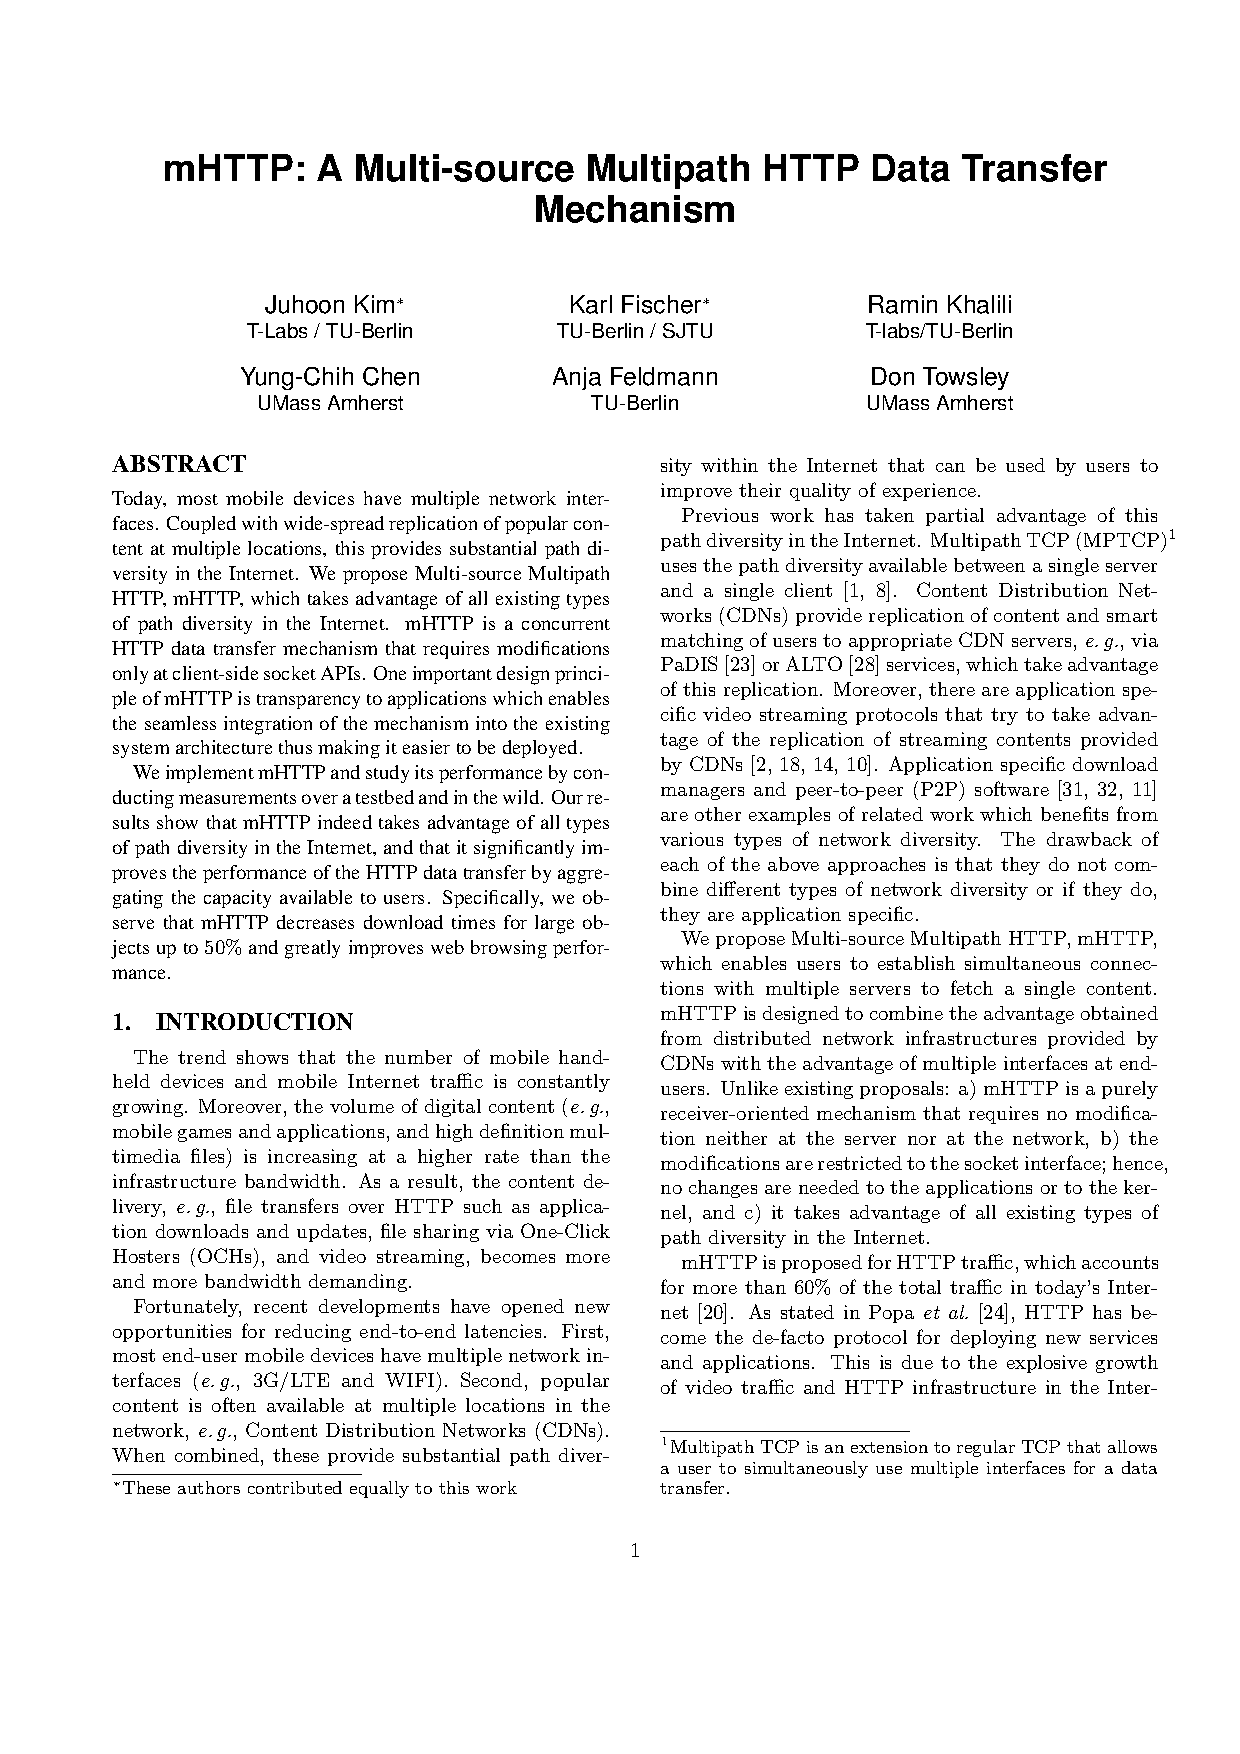
\includepdf[pages=-, offset=75 -75]{Appendices/paper.pdf}

%\input{Appendices/AppendixB}
%\input{Appendices/AppendixC}

\addtocontents{toc}{\vspace{2em}} % Add a gap in the Contents, for aesthetics

\backmatter

%----------------------------------------------------------------------------------------
%	BIBLIOGRAPHY
%----------------------------------------------------------------------------------------

\label{Bibliography}

\lhead{\emph{Bibliography}} % Change the page header to say "Bibliography"

\bibliographystyle{unsrtnat} % Use the "unsrtnat" BibTeX style for formatting the Bibliography

%\bibliography{Bibliography} % The references (bibliography) information are stored in the file named "Bibliography.bib"
\bibliography{main}

\end{document}  
